\section{Results and Discussion}

The full resoults for each test can be found in the folder \href{https://github.com/giovanni-lucarelli/cloud-basic/tree/main/results}{results} in the github repository of the project. Here are briefly discussed only the main ones.

\subsection{HPCC}

The \texttt{hpcc} test has been repeated three times for each environment; here hare reported the mean value ($\pm$ standard deviation) for the main benchmarks, divided by type of metrics.

\subsubsection{Compute Performance}

HPL, DGEMM, and FFT are standard benchmarks or computational kernels used to measure the performance of high-performance computing (HPC) systems, especially with respect to floating-point computation and linear algebra workloads. From the results in table \ref{tab:benchmark_performance} we can see that the container consistently leads or ties with host whereas VMs trails behind in most metrics.
Note in particular the huge difference in performance of the VMs in the MPIFFT. This benchmark requires frequent communication across MPI ranks — often doing all-to-all exchanges for transposing and redistributing FFT data. Other than the capability in crunching numbers this stresses also: Network latency and bandwidth, MPI transport efficiency,  Inter-process communication mechanisms.

The critical difference in the three environment is that, whereas the MPI Communication Mechanism of the host is the shared memory, the container uses TCP network protocol but with low overhead and 
VMs use	TCP over virtual Network Interface Controllers (NICs) that returns very poor latency and bandwidth. MPI runs over virtualized network interfaces, causing massive latency. The ping-pong and iperf tests confirm this as shown in the results in table \ref{tab:pingpong} and \ref{tab:iperf}.

\begin{table}[htbp]
\centering

\renewcommand{\arraystretch}{1.2}
\begin{tabular}{lccc}
\toprule
\textbf{Benchmark} & \textbf{VM} & \textbf{Container} & \textbf{Host} \\
\midrule
\textbf{HPL (Gflops)} & 5.128 ± 0.013 & 5.552 ± 0.034 & 5.516 ± 0.027 \\
\midrule
\textbf{DGEMM (Gflops)} & & & \\
StarDGEMM     & 1.290 ± 0.045 & 1.303 ± 0.122 & 1.400 ± 0.005 \\
SingleDGEMM   & 1.907 ± 0.077 & 2.081 ± 0.052 & 2.054 ± 0.024 \\
\midrule
\textbf{FFT (Gflops)} & & & \\
StarFFT      & 1.453 ± 0.033 & 1.832 ± 0.025 & 1.816 ± 0.008 \\
SingleFFT    & 2.638 ± 0.047 & 2.767 ± 0.054 & 2.739 ± 0.141 \\
MPIFFT       & 1.231 ± 0.064 & 3.673 ± 0.124 & 4.042 ± 0.014 \\
\bottomrule
\end{tabular}
\caption{Benchmark performance (in Gflops) across the three execution environments. Values are reported as mean ± standard deviation, calculated over three measurements ($n = 3$).}
\label{tab:benchmark_performance}
\end{table}

\begin{figure}[H]
    \centering
    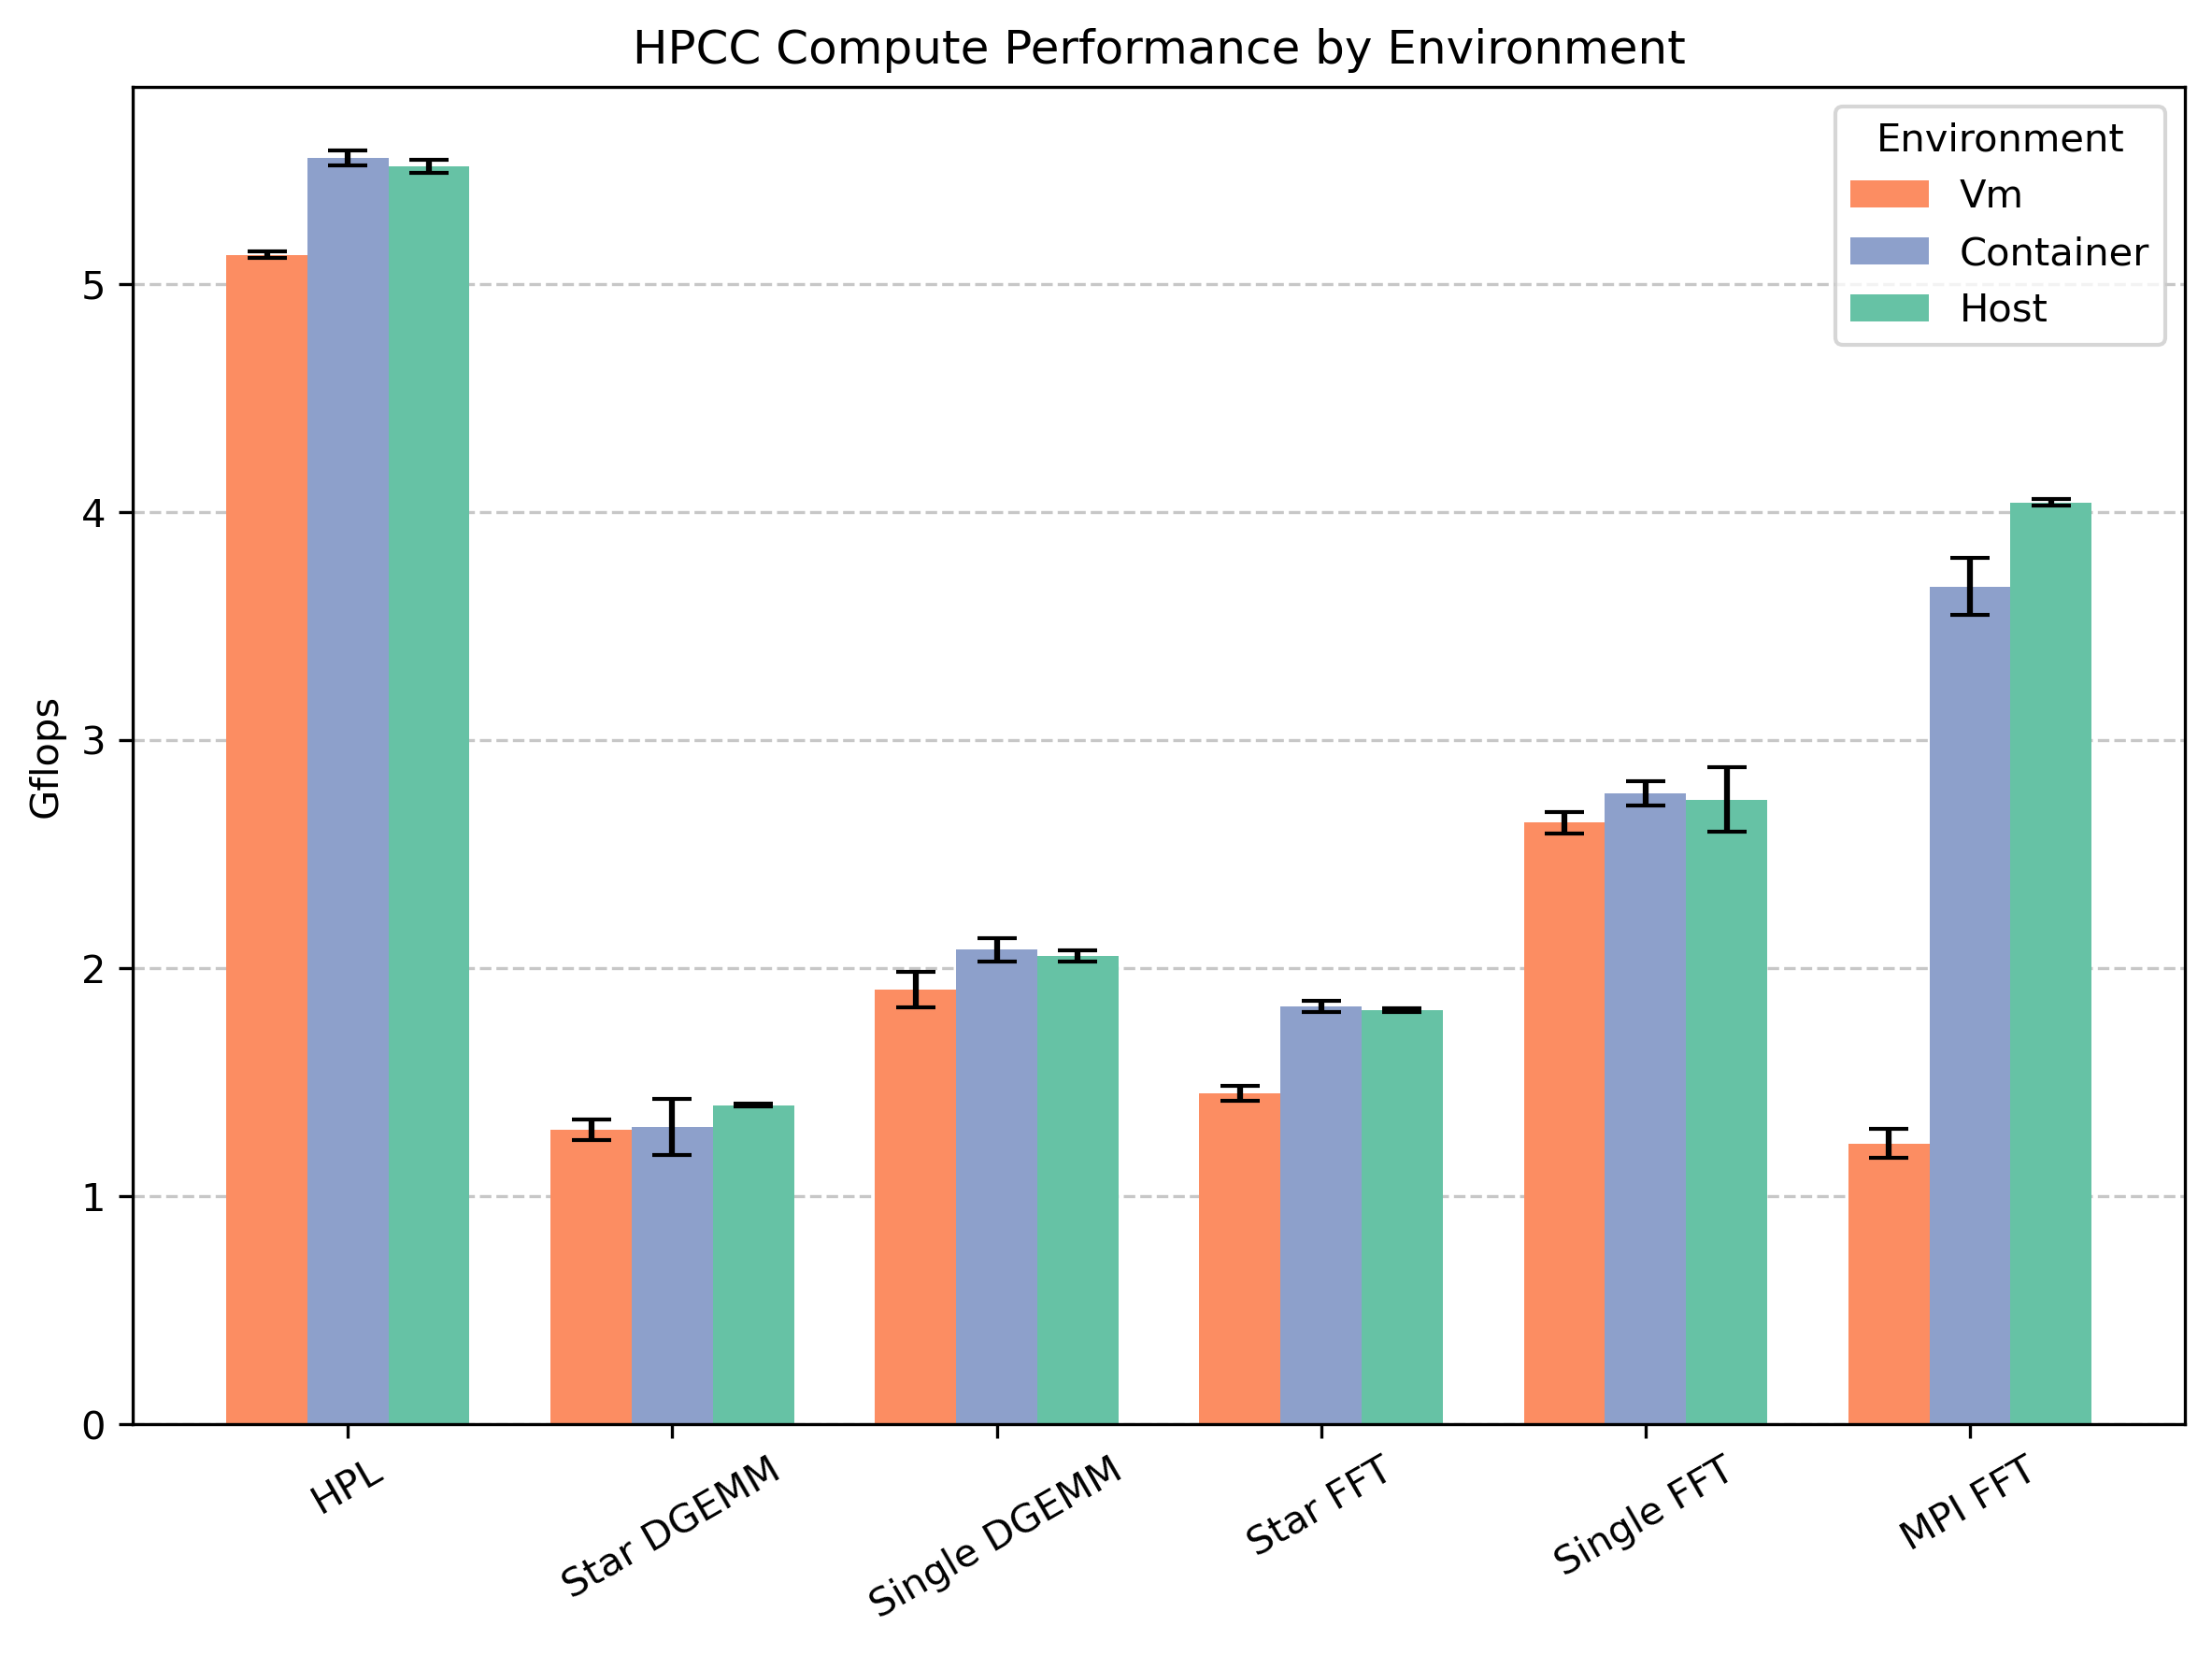
\includegraphics[width=0.8\linewidth]{assets/hpcc_compute_performance.png}
    \caption{Caption}
    \label{fig:hpcc_compute_performance}
\end{figure}

\subsubsection{Memory Benchmarks}

The STREAM benchmark provides a measure of the memory bandwidth (GB/s) by testing simple vector operations like Copy, Scale, Add, and Triad. \textbf{Single} on a single processor node and \textbf{Star} Measures aggregate memory bandwidth across the system using multiple nodes.

Memory Bandwidth (STREAM): Host and container perform similarly, with VM being the weakest.
A note on the SingleSTREAM, we can see that SingleSTREAM reach a good amount of the nominal memory bandwidth in all the environment.

Looking at the nominal performance. By running the command: \texttt{sudo dmidecode --type memory}:

\begin{minted}{text}
Configured Memory Speed: 1867 MT/s
Number of memory bank: 2
\end{minted}

\begin{equation*}
    \text{BW}_\text{nom} = 1.867 \frac{\text{GT}}{\text{s}}\times 8\,\frac{\text{B}}{\text{T}}\times 2 = 29.872 \frac{\text{GB}}{\text{s}}
\end{equation*}

the Copy benchmark\footnote{in particular the Copy benchmark because it is the more optimized by the compiler with an assemply written function!} is pretty satisfiyng for all the environments: vm 75\%, container 0.81\%, host 0.78\% ot the nominal bandwidth. 

StarSTREAM, running across the two nodes in the VM and Container clusters, is measuring a distributed memory benchmark. This involves significant inter-node communication to exchange data required by the benchmark kernels. The bandwidth in this scenario is not limited by the speed of local memory access but by the speed and latency of the network (or virtual network) connecting the two nodes. The process of sending and receiving data over the network, along with any necessary synchronization and coordination between the nodes, introduces substantial overhead. This overhead drastically reduces the effective memory bandwidth seen by the application, resulting in the much lower figures (around $20\%$ of nominal).


The RandomAccess benchmark measures the rate of random updates to memory (UP/s). It's designed to stress the memory system's ability to handle a large number of small, non-contiguous memory accesses. This is different from STREAM, which focuses on large, sequential data transfers. 
The MPI Random Access has an interesting behaviour: the Host results are largely out of scale, this can be interpreted thinking at the fact that in vms and containers the mpi protocol is managed through the network adapter and so using the TCP protocol, where as in the host we are in the context of shared memory. MPI processes can use shared memory for inter-process communication, which is orders of magnitude faster than network-based communication This is backed up by the ping pong latency benchmarks. for the vms the latency is much higher, consistent with virtual NIC and TCP stack overhead.

PTRANS (Parallel Matrix Transpose) is designed to measure the global network bandwidth (GB/s) in a parallel computing system. Specifically, it assesses the rate at which large arrays of data can be transferred between the memories of different processors in the system.
This shows huge performance difference expecially the VMs compared to the other environment, probably due to the already mentioned network bottleneck.



\begin{table}[H]
\centering
\renewcommand{\arraystretch}{1.2}
\begin{tabular}{lccc}
\toprule
\textbf{Benchmark} & \textbf{VM} & \textbf{Container} & \textbf{Host} \\
\midrule
\textbf{SingleSTREAM (GB/s)} & & & \\
Copy   & 22.30 ± 0.32 & 24.11 ± 0.20 & 23.44 ± 0.06 \\
Scale  & 13.26 ± 0.19 & 14.23 ± 0.06 & 14.06 ± 0.12 \\
Add    & 14.40 ± 0.24 & 15.38 ± 0.16 & 15.06 ± 0.14 \\
Triad  & 14.44 ± 0.28 & 15.48 ± 0.13 & 15.22 ± 0.05 \\
\midrule
\textbf{StarSTREAM (GB/s)} & & & \\
Copy   & 5.03 ± 0.03 & 5.41 ± 0.03 & 5.39 ± 0.02 \\
Scale  & 3.34 ± 0.03 & 3.55 ± 0.01 & 3.56 ± 0.01 \\
Add    & 3.75 ± 0.01 & 4.08 ± 0.02 & 4.07 ± 0.01 \\
Triad  & 3.72 ± 0.04 & 4.02 ± 0.02 & 4.00 ± 0.02 \\
\midrule
\textbf{RandomAccess (MUP/s)} & & & \\
MPI\_LCG     & 2.25 ± 0.02 & 2.64 ± 0.42 & 34.25 ± 0.30 \\
MPI          & 2.29 ± 0.02 & 2.60 ± 0.54 & 31.58 ± 0.51 \\
Star\_LCG    & 5.71 ± 0.03 & 13.85 ± 2.17 & 14.29 ± 0.39 \\
Single\_LCG  & 23.82 ± 1.93 & 41.92 ± 9.47 & 47.40 ± 5.16 \\
Star         & 5.54 ± 0.10 & 13.23 ± 2.06 & 13.21 ± 0.20 \\
Single       & 25.56 ± 2.23 & 44.71 ± 9.66 & 46.89 ± 2.46 \\
\midrule
\textbf{PTRANS (GB/s)} & 0.196 ± 0.014 & 1.181 ± 0.239 & 1.495 ± 0.019 \\
\bottomrule
\end{tabular}
\caption{Memory Bandwidth Benchmarks: VM vs Container vs Host (GB/s)}
\end{table}

\begin{figure}[H]
    \centering
    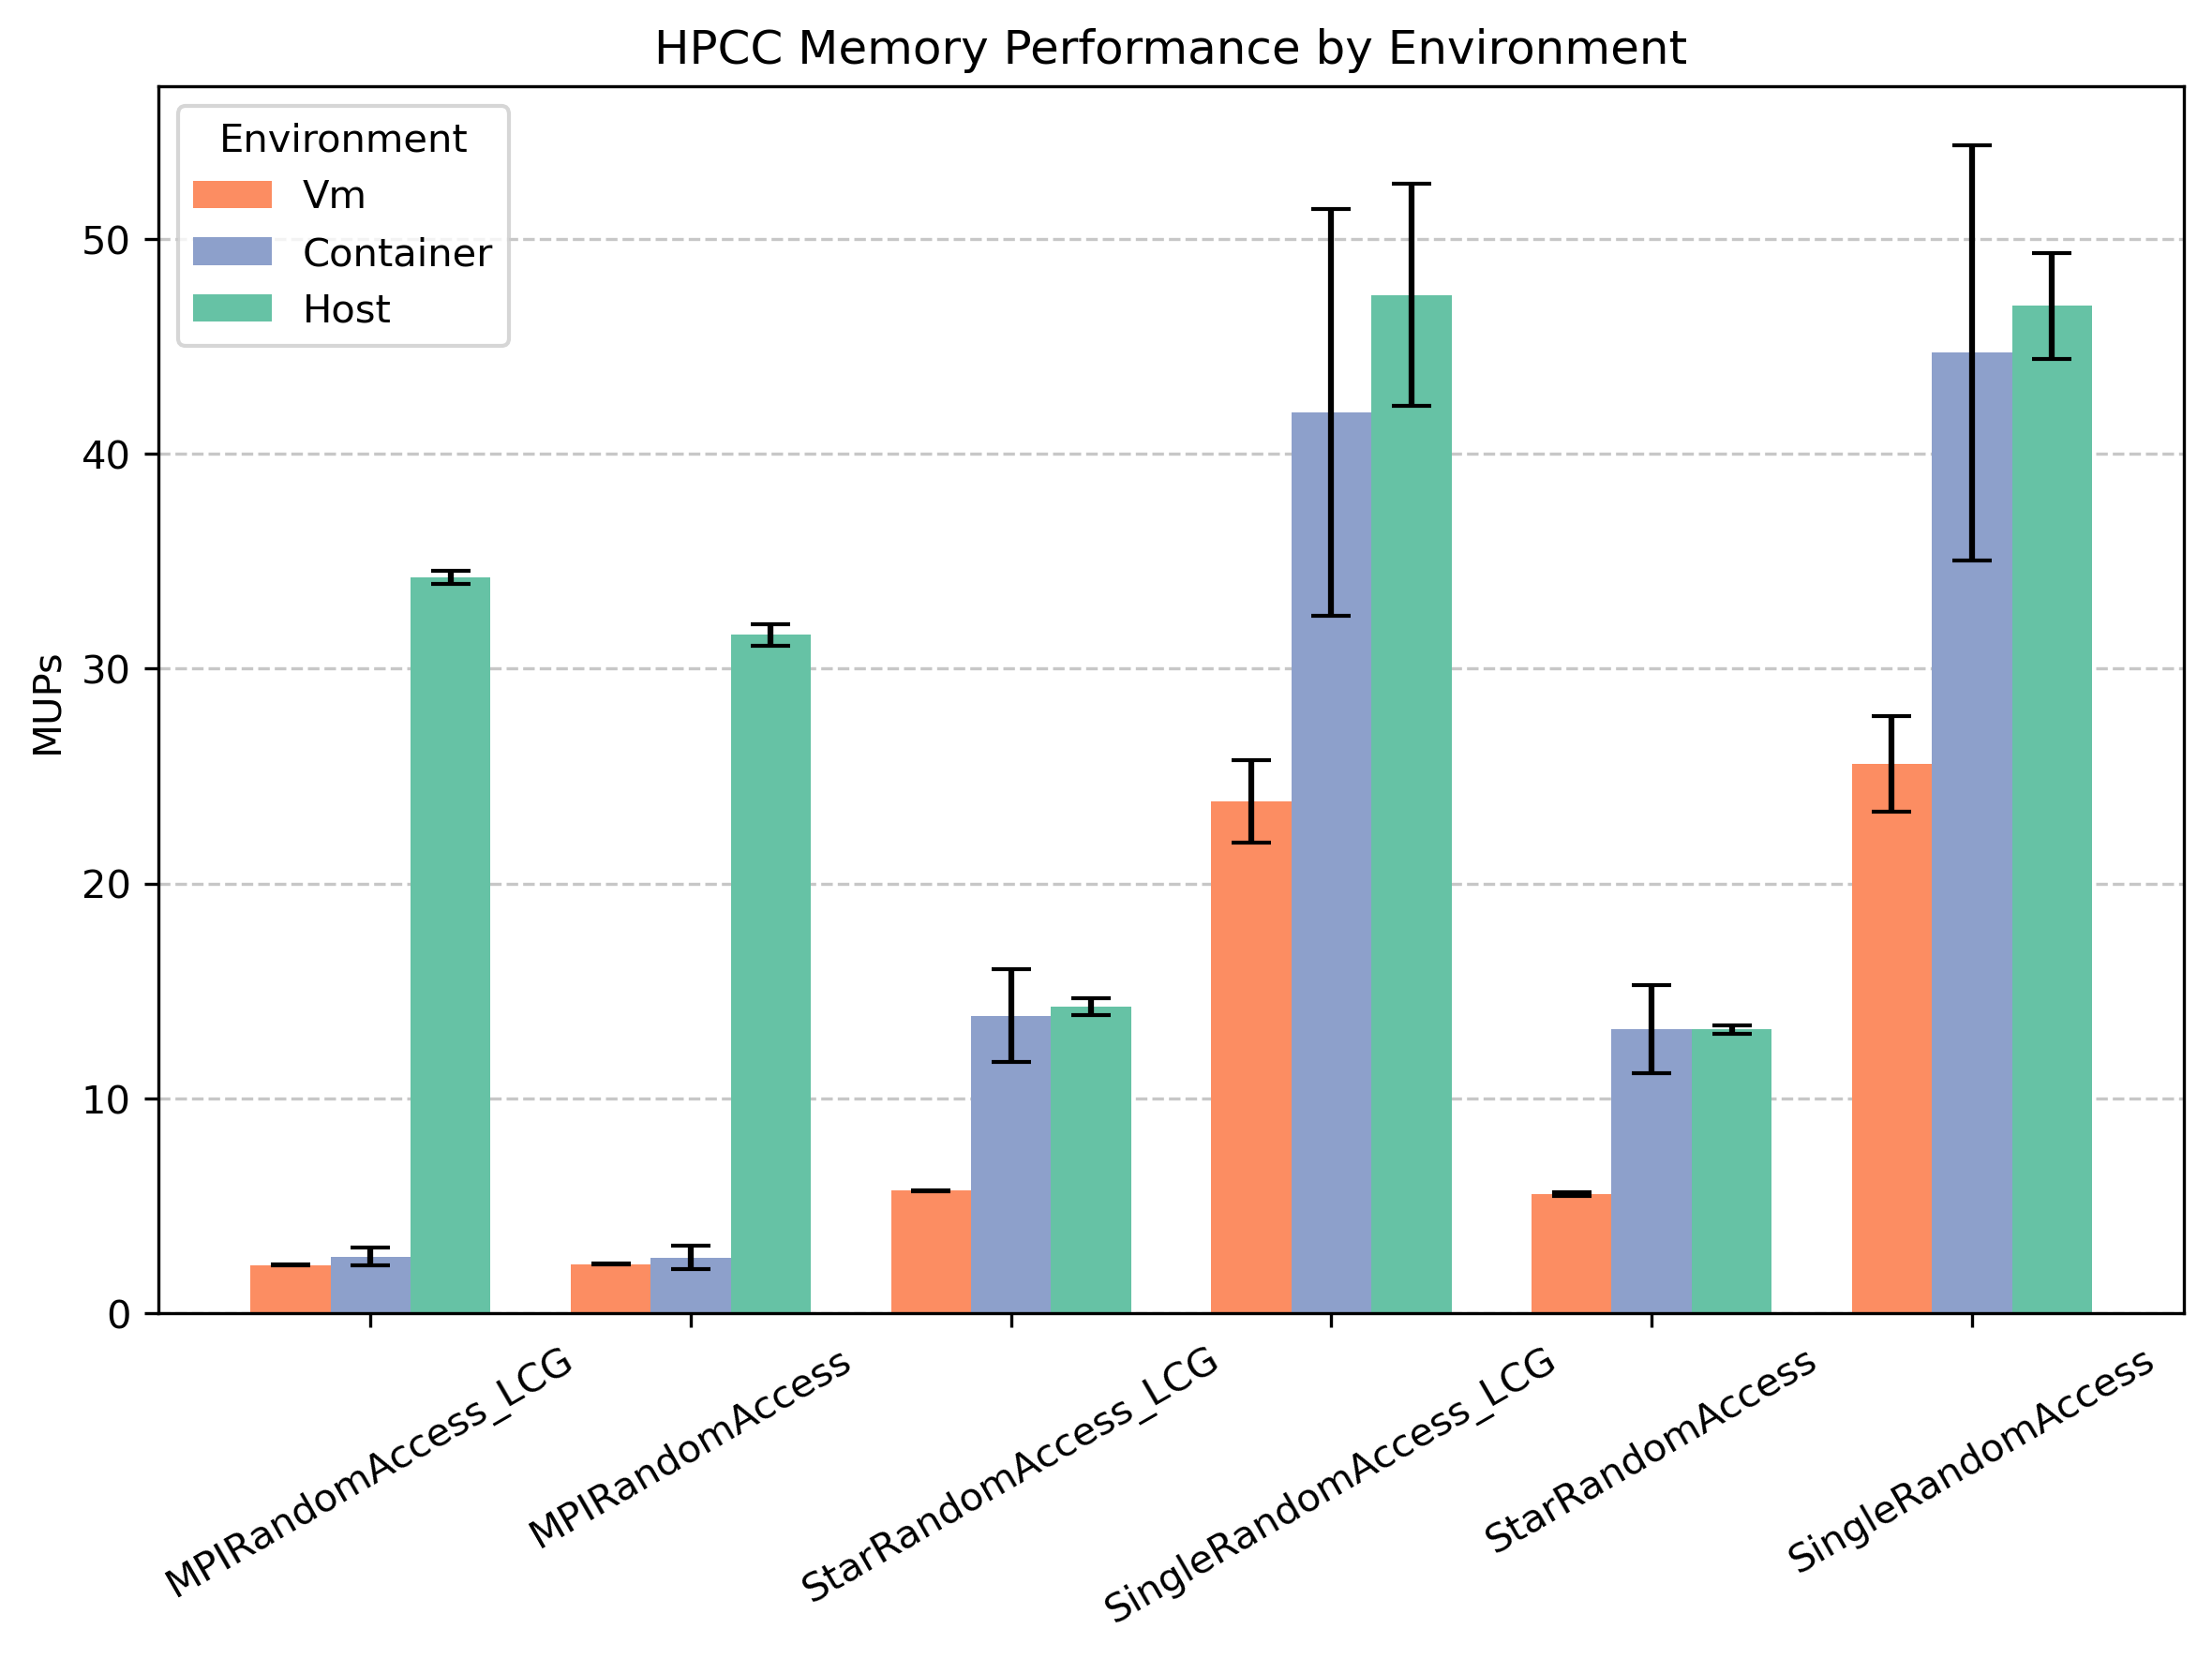
\includegraphics[width=0.8\linewidth]{assets/hpcc_memory_performance.png}
    \caption{Caption}
    \label{fig:hpcc_memory_performance}
\end{figure}

\subsubsection{Latency and Bandwidth}

The ping-pong benchmark is a fundamental test used to measure the performance of a communication channel or link between two endpoints.
In a cluster environment, a ping-pong benchmark is typically run between two different nodes. On a single host machine, a ping-pong benchmark is typically run between two processes or threads running on that same machine. For this reason here the Host results are not a proper baseline to compare the VMs and container results.

From the table \ref{tab:pingpong} we can see that VM introduces massive latency penalties with respect to the Containers. Analogously, for the bandwidth the containers show the best performances.

\begin{table}[H]
\centering
\renewcommand{\arraystretch}{1.2}
\begin{tabular}{lccc}
\toprule
\textbf{Benchmark} & \textbf{VM} & \textbf{Container} & \textbf{Host} \\
\midrule
\multicolumn{4}{l}{\textbf{Latency (µs)}} \\
MinPingPong             & 1.957 ± 0.066 & 1.853 ± 0.056 & 0.201 ± 0.004 \\
AvgPingPong              & 49.026 ± 1.597 & 6.855 ± 0.600 & 0.211 ± 0.005 \\
MaxPingPong              & 75.651 ± 2.980 & 9.962 ± 1.540 & 0.218 ± 0.004 \\
NaturallyOrderedRing    & 61.426 ± 7.146 & 5.926 ± 0.376 & 0.227 ± 0.005 \\
RandomlyOrderedRing     & 63.771 ± 8.449 & 6.872 ± 0.332 & 0.230 ± 0.003 \\
\midrule
\multicolumn{4}{l}{\textbf{Bandwidth (GB/s)}} \\
MinPingPong            & 0.230 ± 0.025 & 4.995 ± 1.033 & 11.517 ± 0.725 \\
AvgPingPong            & 3.617 ± 0.422 & 7.943 ± 0.674 & 12.750 ± 0.212 \\
MaxPingPong            & 11.383 ± 1.381 & 13.726 ± 0.278 & 13.908 ± 0.468 \\
NaturallyOrderedRing  & 0.145 ± 0.020 & 2.064 ± 0.115 & 3.101 ± 0.021 \\
RandomlyOrderedRing   & 0.120 ± 0.014 & 1.857 ± 0.020 & 2.971 ± 0.073 \\
\bottomrule
\end{tabular}
\label{tab:pingpong}
\caption{Latency and Bandwidth Benchmarks: VM vs Container vs Host}

\end{table}

\begin{figure}[H]
    \centering
    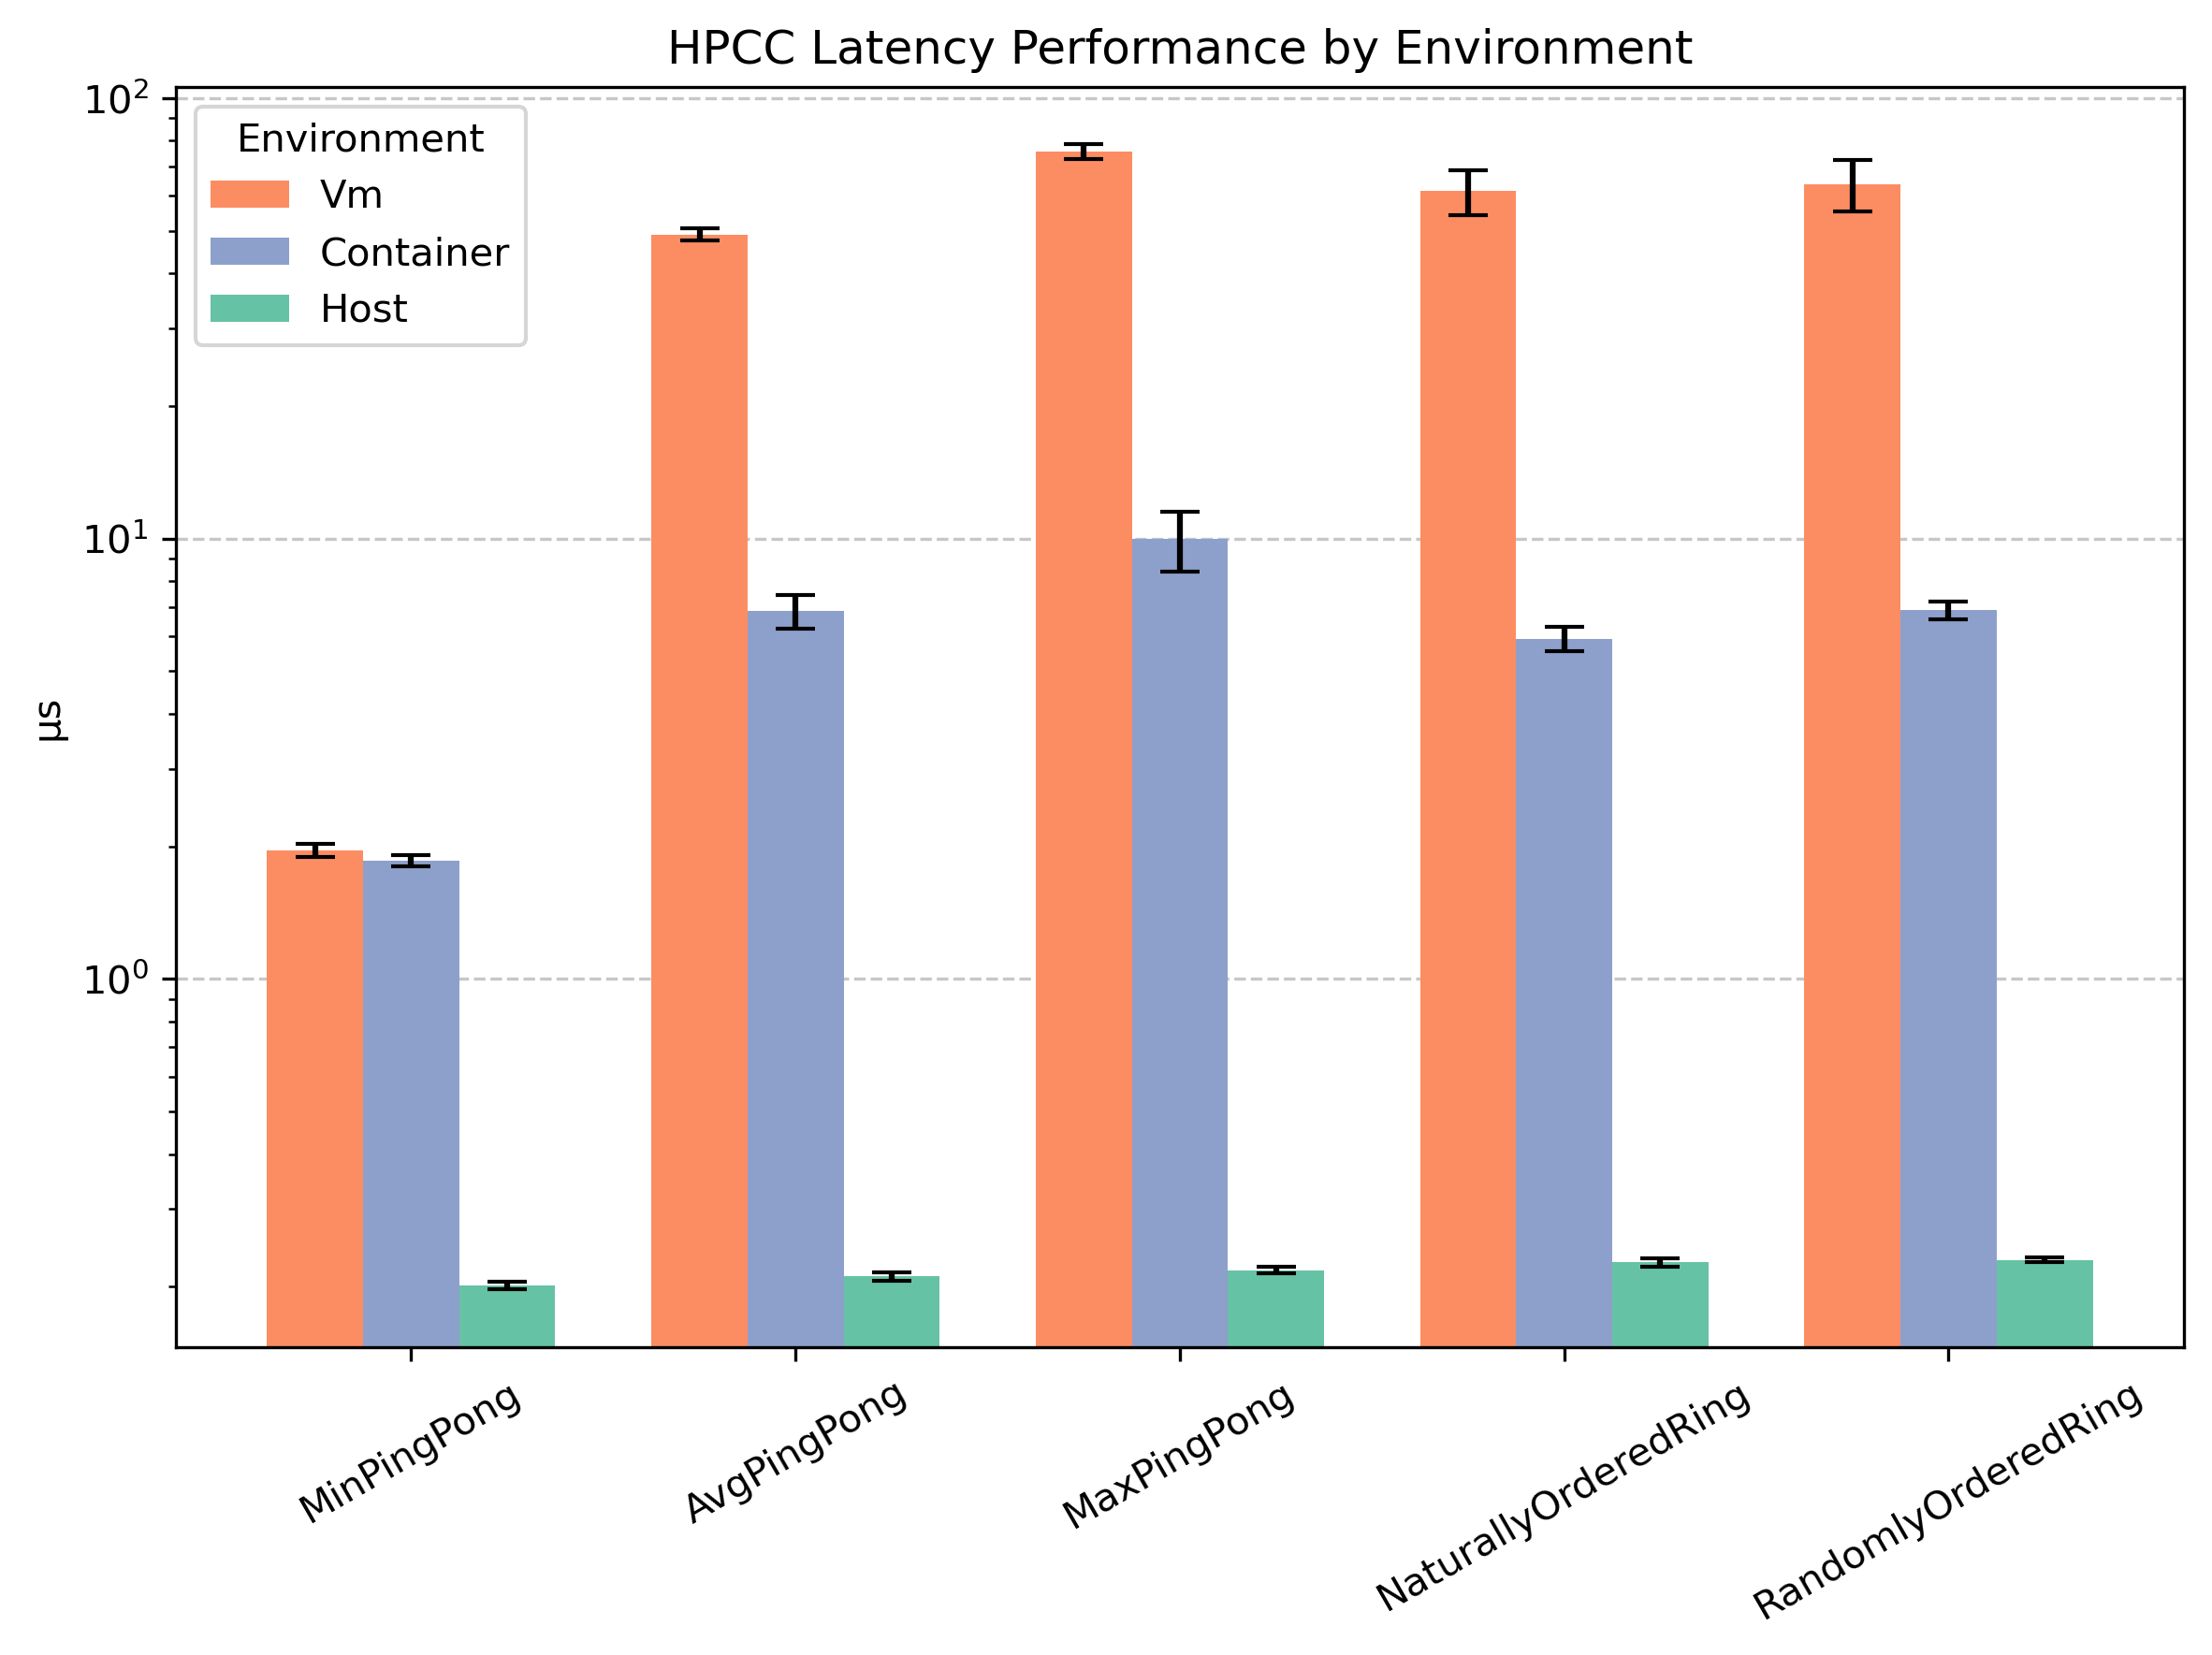
\includegraphics[width=0.8\linewidth]{assets/hpcc_latency_performance.png}
    \caption{Note the log scale}
    \label{fig:hpcc_latency_performance}
\end{figure}

\subsection{stress-ng}

From the stress-ng documentation\footnote{\url{https://wiki.ubuntu.com/Kernel/Reference/stress-ng}}: `` Stress-ng measures a stress test ``throughput" using ``bogus operations per second". The size of a bogo op depends on the stressor being run, and are not comparable between different stressors.''

Regarding the cpu stressor, host and container shows nearly identical performances, the light variability is negligible and is inside the variability of the tests. VMs throughput performances are significantly lower, about the $31\%$ lower than host/container. This is probably due to the virtual overhead introduced by the hypervisor.

Similiarly to the cpu, for the memory stressor the VM results are again the lowest, significantly lower than host and container, again similiar. 
Real Time (Wall-Clock Time) is the total time that elapsed from when the benchmark started until it finished, as measured by a clock on the wall, Usr+Sys Time (CPU Time) is the total amount of CPU time that the benchmark process spent executing code.
The large difference between Real Time and Usr+Sys Time for the Container and Host in the Memory VM stressor is the expected result of running a multi-threaded benchmark effectively utilizing multiple CPU cores. The absence of this large difference in the VM environment highlights that the virtualization layer in VirtualBox introduces overhead or inefficiencies that hinder the effective parallel execution and CPU utilization of this specific memory-intensive multi-threaded workload compared to running it directly on the host or within a Docker container.

\begin{table}[H]
    \centering
    \begin{tabular}{lccc}
    \toprule
    \textbf{Benchmark} & \textbf{VM} & \textbf{Container} & \textbf{Host} \\
    \midrule
    \textbf{CPU (kBOps/s)} & & & \\
    Real Time & $0.924 \pm 0.008$ & $1.340 \pm 0.013$ & $1.348 \pm 0.016$ \\
    Usr+Sys Time & $0.926 \pm 0.008$ & $1.342 \pm 0.013$ & $1.349 \pm 0.016$ \\
    \midrule
    \textbf{Memory (kBOps/s)} & & & \\
    Real Time & $40.183 \pm 0.265$ & $52.180 \pm 5.025$ & $53.900 \pm 4.948$ \\
    Usr+Sys Time & $41.434 \pm 0.952$ & $66.543 \pm 2.954$ & $62.687 \pm 3.254$ \\
    \bottomrule
    \end{tabular}
    \caption{kilo BogoOps/s for each benchmark, number of repetition of the experiment $n=5$}
    \label{tab:stress-ng}
\end{table}
\subsection{sysbench}
%TODO: restyle
CPU Performance: The CPU performance per node is largely uniform across all three environments in terms of average metrics. The addition of maximum latency shows that the single Host is slightly more stable in avoiding high-latency CPU events compared to the clustered environments (VM and Container). The total latency sum is dominated by the test duration. For typical CPU workloads, there's no significant advantage or disadvantage to using VMs or Containers in a cluster compared to a single host based on these results.
Memory Performance: This is where the significant differences lie. The Container cluster setup provides superior memory throughput per node compared to both the VM cluster and the single Host. The VM cluster exhibits a considerable performance bottleneck for memory operations. The single Host is a solid performer but doesn't reach the peak memory throughput of the Container node. The maximum latency metric suggests slightly less predictability in memory access times within the clustered environments compared to the single host, although the differences are relatively small. The sum of latencies strongly supports the Container's efficiency and the VM's inefficiency in memory handling.

\begin{table}[H]
    \centering
    \begin{tabular}{lccc}
    \toprule
    \textbf{Benchmark} & \textbf{VM} & \textbf{Container} & \textbf{Host} \\
    \midrule
    \textbf{CPU} & & & \\
    Events/s & $453.97 \pm 1.28$ & $459.74 \pm 2.54$ & $452.38 \pm 6.76$ \\
    Latency min (ms) & $2.04 \pm 0.01$ & $2.03 \pm 0.00$ & $2.05 \pm 0.02$ \\
    Latency avg (ms) & $2.20 \pm 0.01$ & $2.17 \pm 0.01$ & $2.21 \pm 0.03$ \\
    Latency max (ms) & $6.05 \pm 1.18$ & $6.14 \pm 2.73$ & $5.49 \pm 1.56$ \\
    Latency sum (ms) & $9998.15 \pm 0.70$ & $9999.55 \pm 0.51$ & $9999.56 \pm 0.72$ \\
    \midrule
    \textbf{Memory} & & & \\
    Transfer rate (Gib/s) & $3.88 \pm 0.02$ & $5.51 \pm 0.09$ & $5.19 \pm 0.08$ \\
    Latency max (ms) & $1.26 \pm 0.50$ & $1.32 \pm 0.62$ & $1.09 \pm 0.24$ \\
    Latency sum (ms) & $1066.09 \pm 8.01$ & $839.99 \pm 14.63$ & $895.79 \pm 18.40$ \\
    \bottomrule

    \end{tabular}
    \caption{Caption}
    \label{tab:sysbench}
\end{table}


\subsection{IOZone}
% TODO: write comparison
% TODO: add the host machine data to compare
% TODO: add a table for a fixen filesize to compare in read/write thre three environment

For clarity the plots of the host are not reported(?) but can be found here.
\begin{figure}[H]
    \centering
    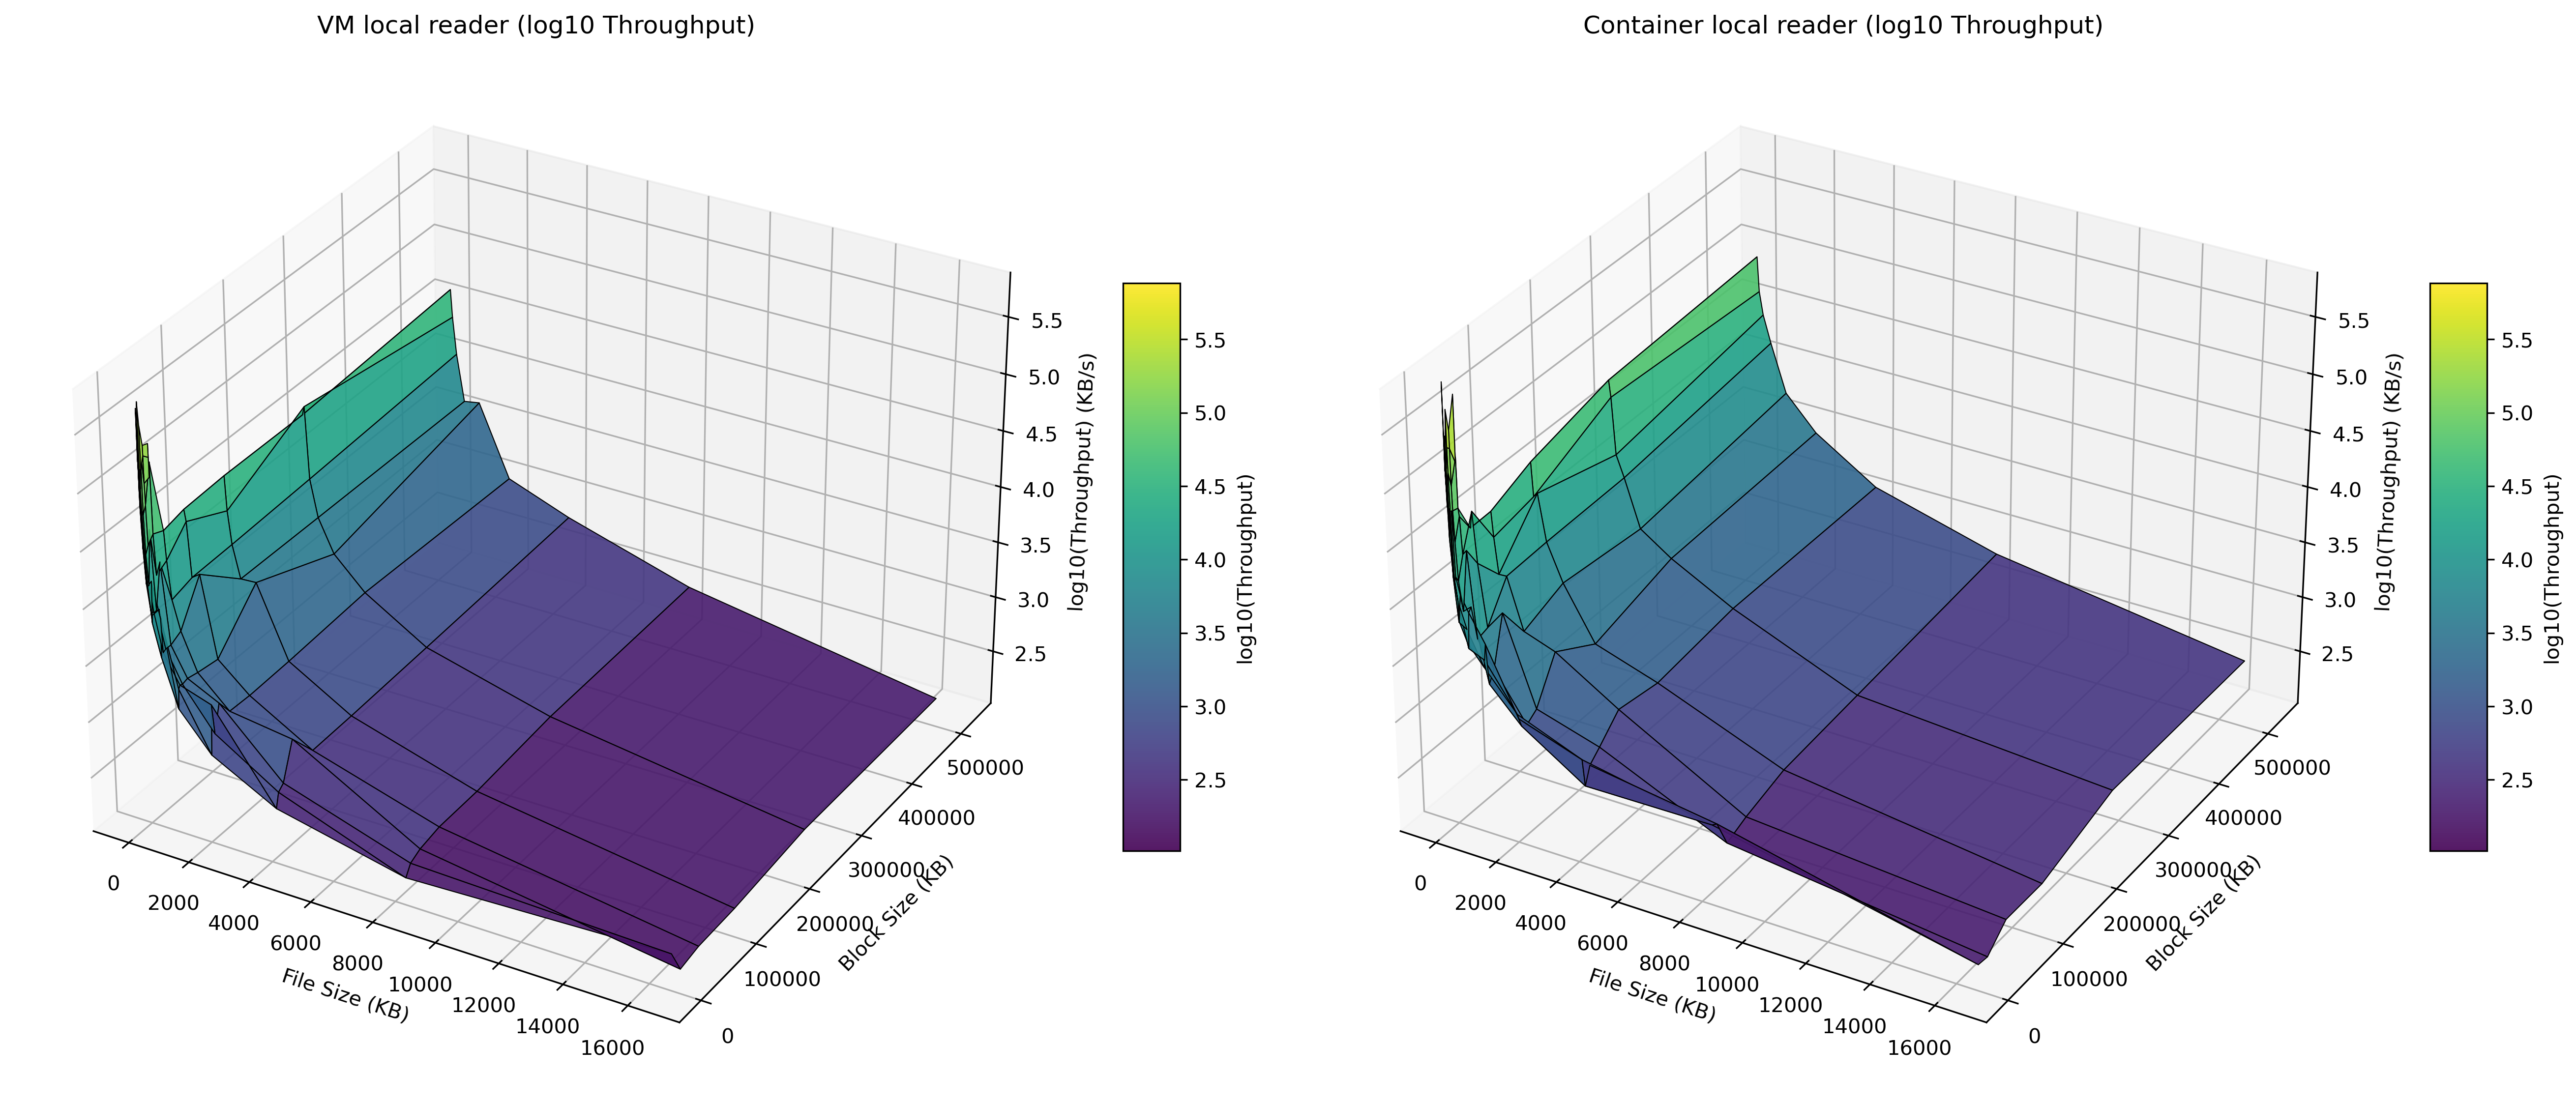
\includegraphics[width=\linewidth]{assets/VM local reader_Container local reader_log_surfaces.png}
    \end{figure}
\begin{figure}[H]
    \centering
    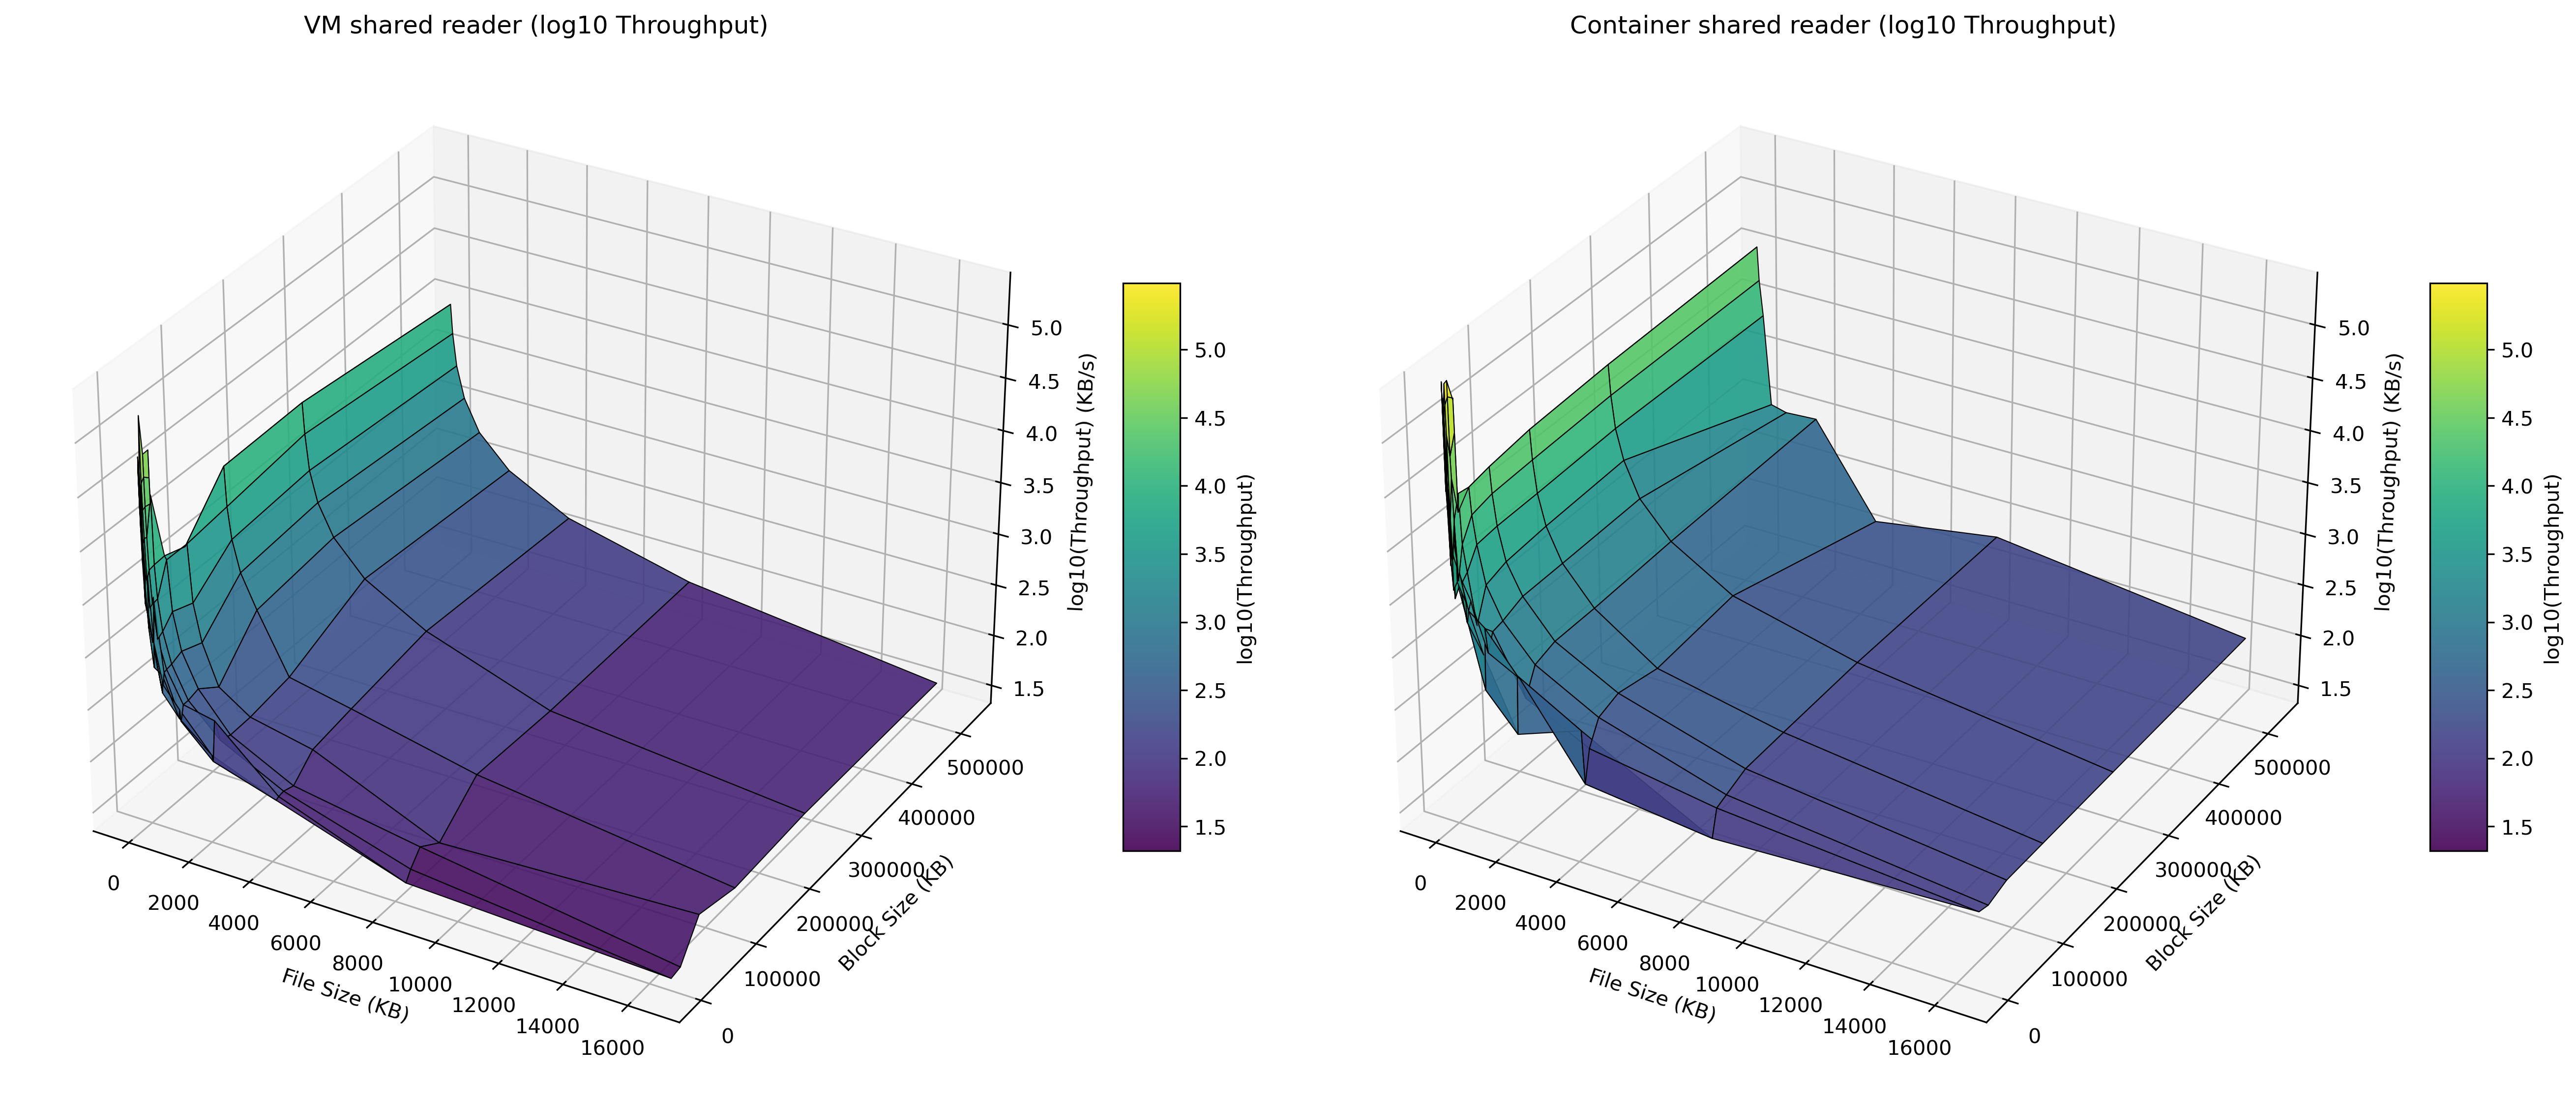
\includegraphics[width=\linewidth]{assets/VM shared reader_Container shared reader_log_surfaces.png}
    \caption{local and shared reader report}
    \label{fig:reader local and shared}
\end{figure}

\begin{figure}[H]
    \centering
    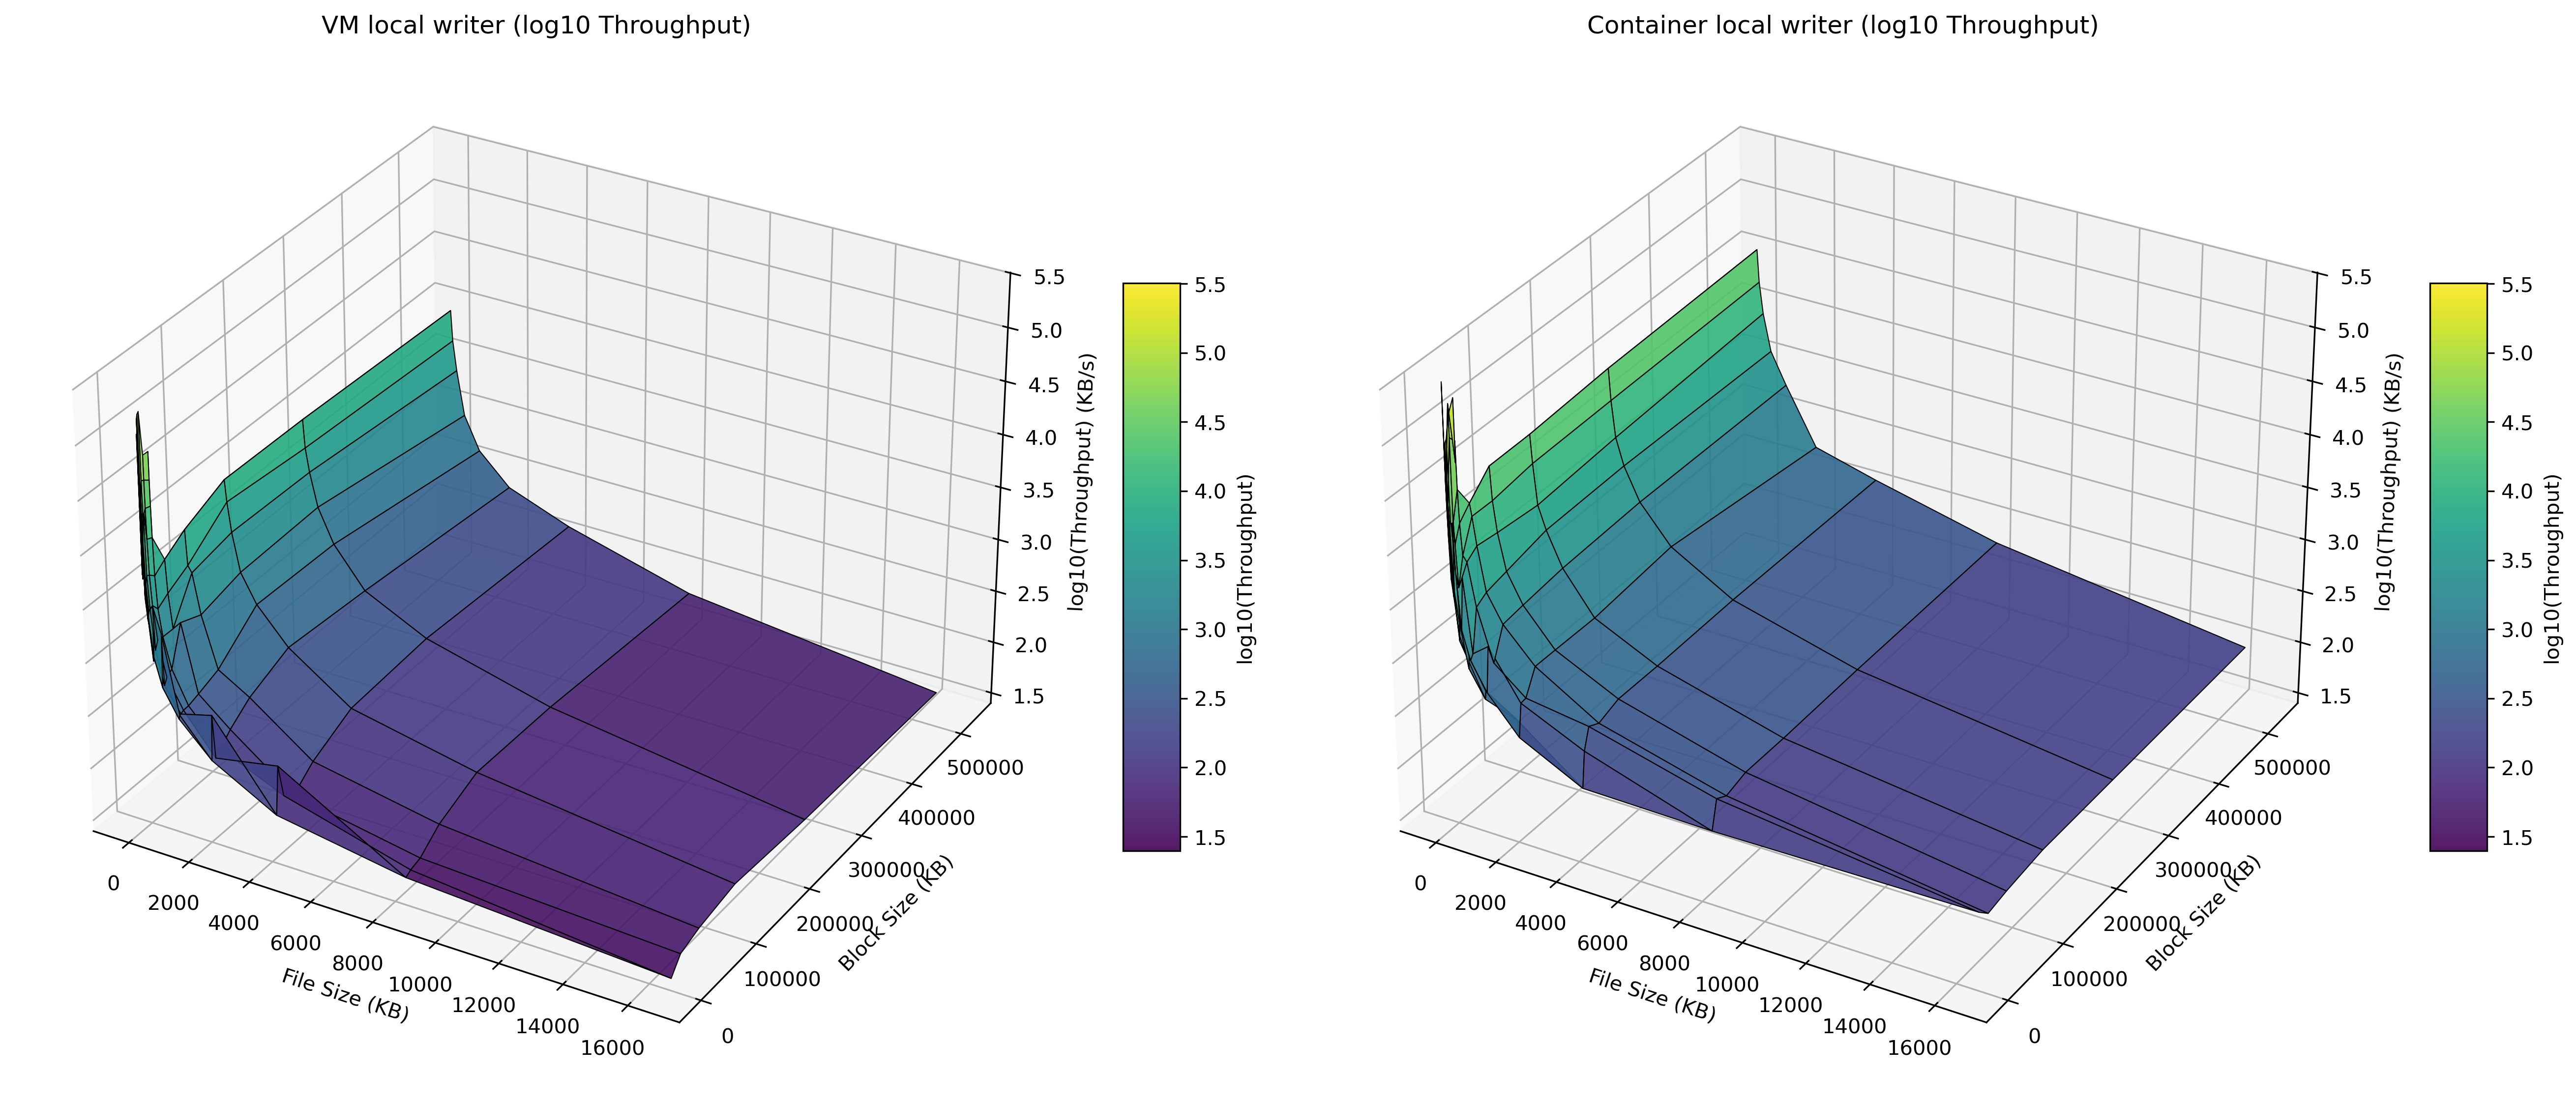
\includegraphics[width=\linewidth]{assets/VM local writer_Container local writer_log_surfaces.png}
        \end{figure}
\begin{figure}[H]
    \centering
    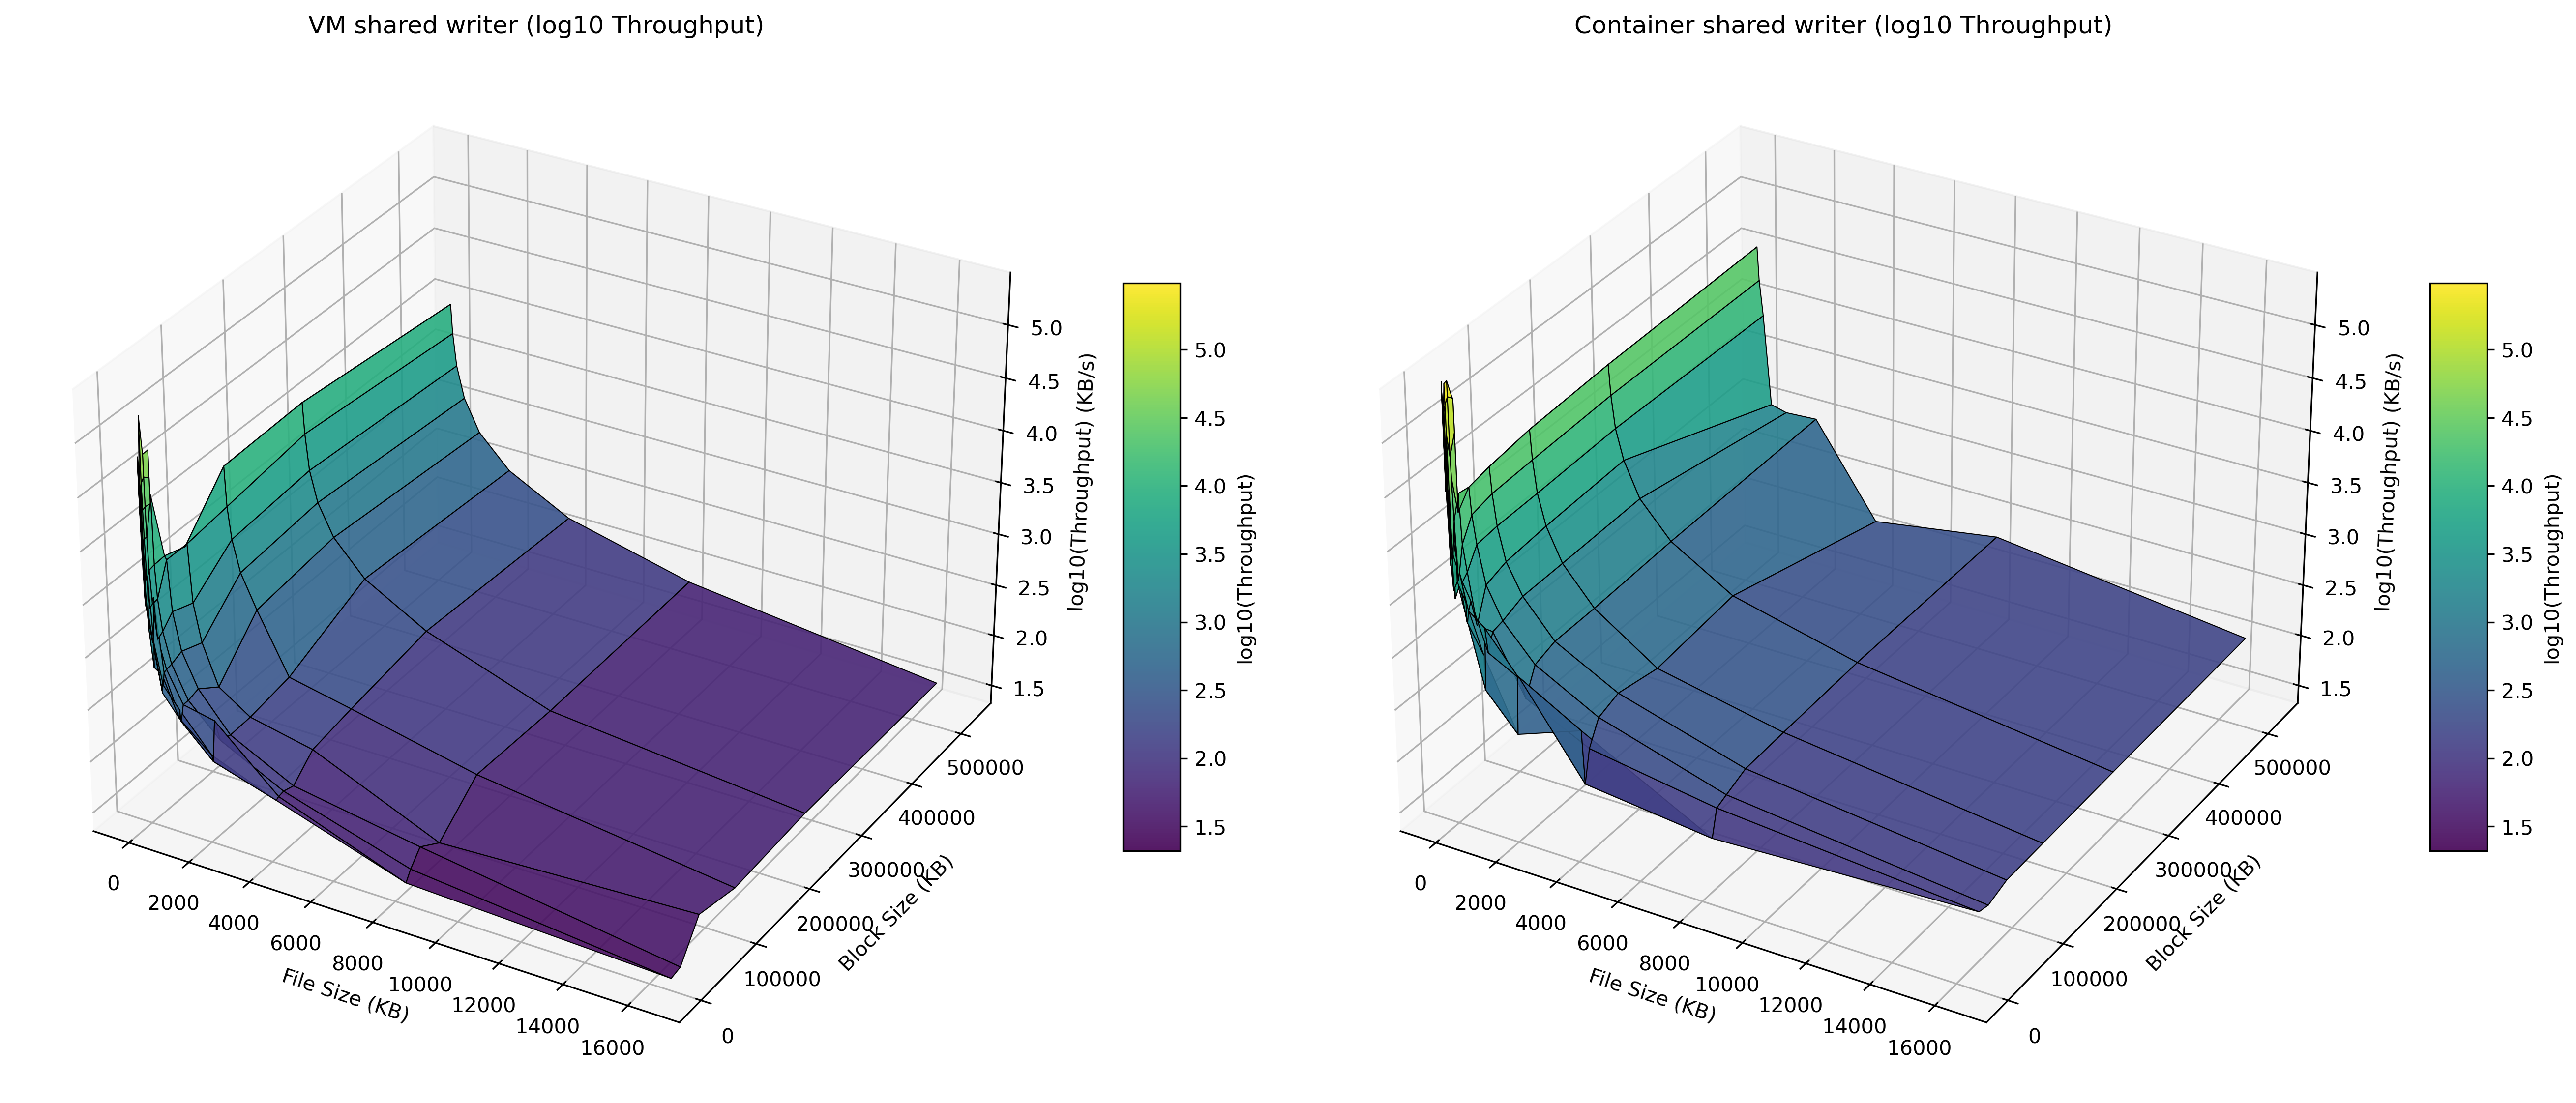
\includegraphics[width=\linewidth]{assets/VM shared writer_Container shared writer_log_surfaces.png}
    \caption{local and shared writer report}
    \label{fig:writer local and shared}
\end{figure}

\begin{figure}[H]
    \centering
    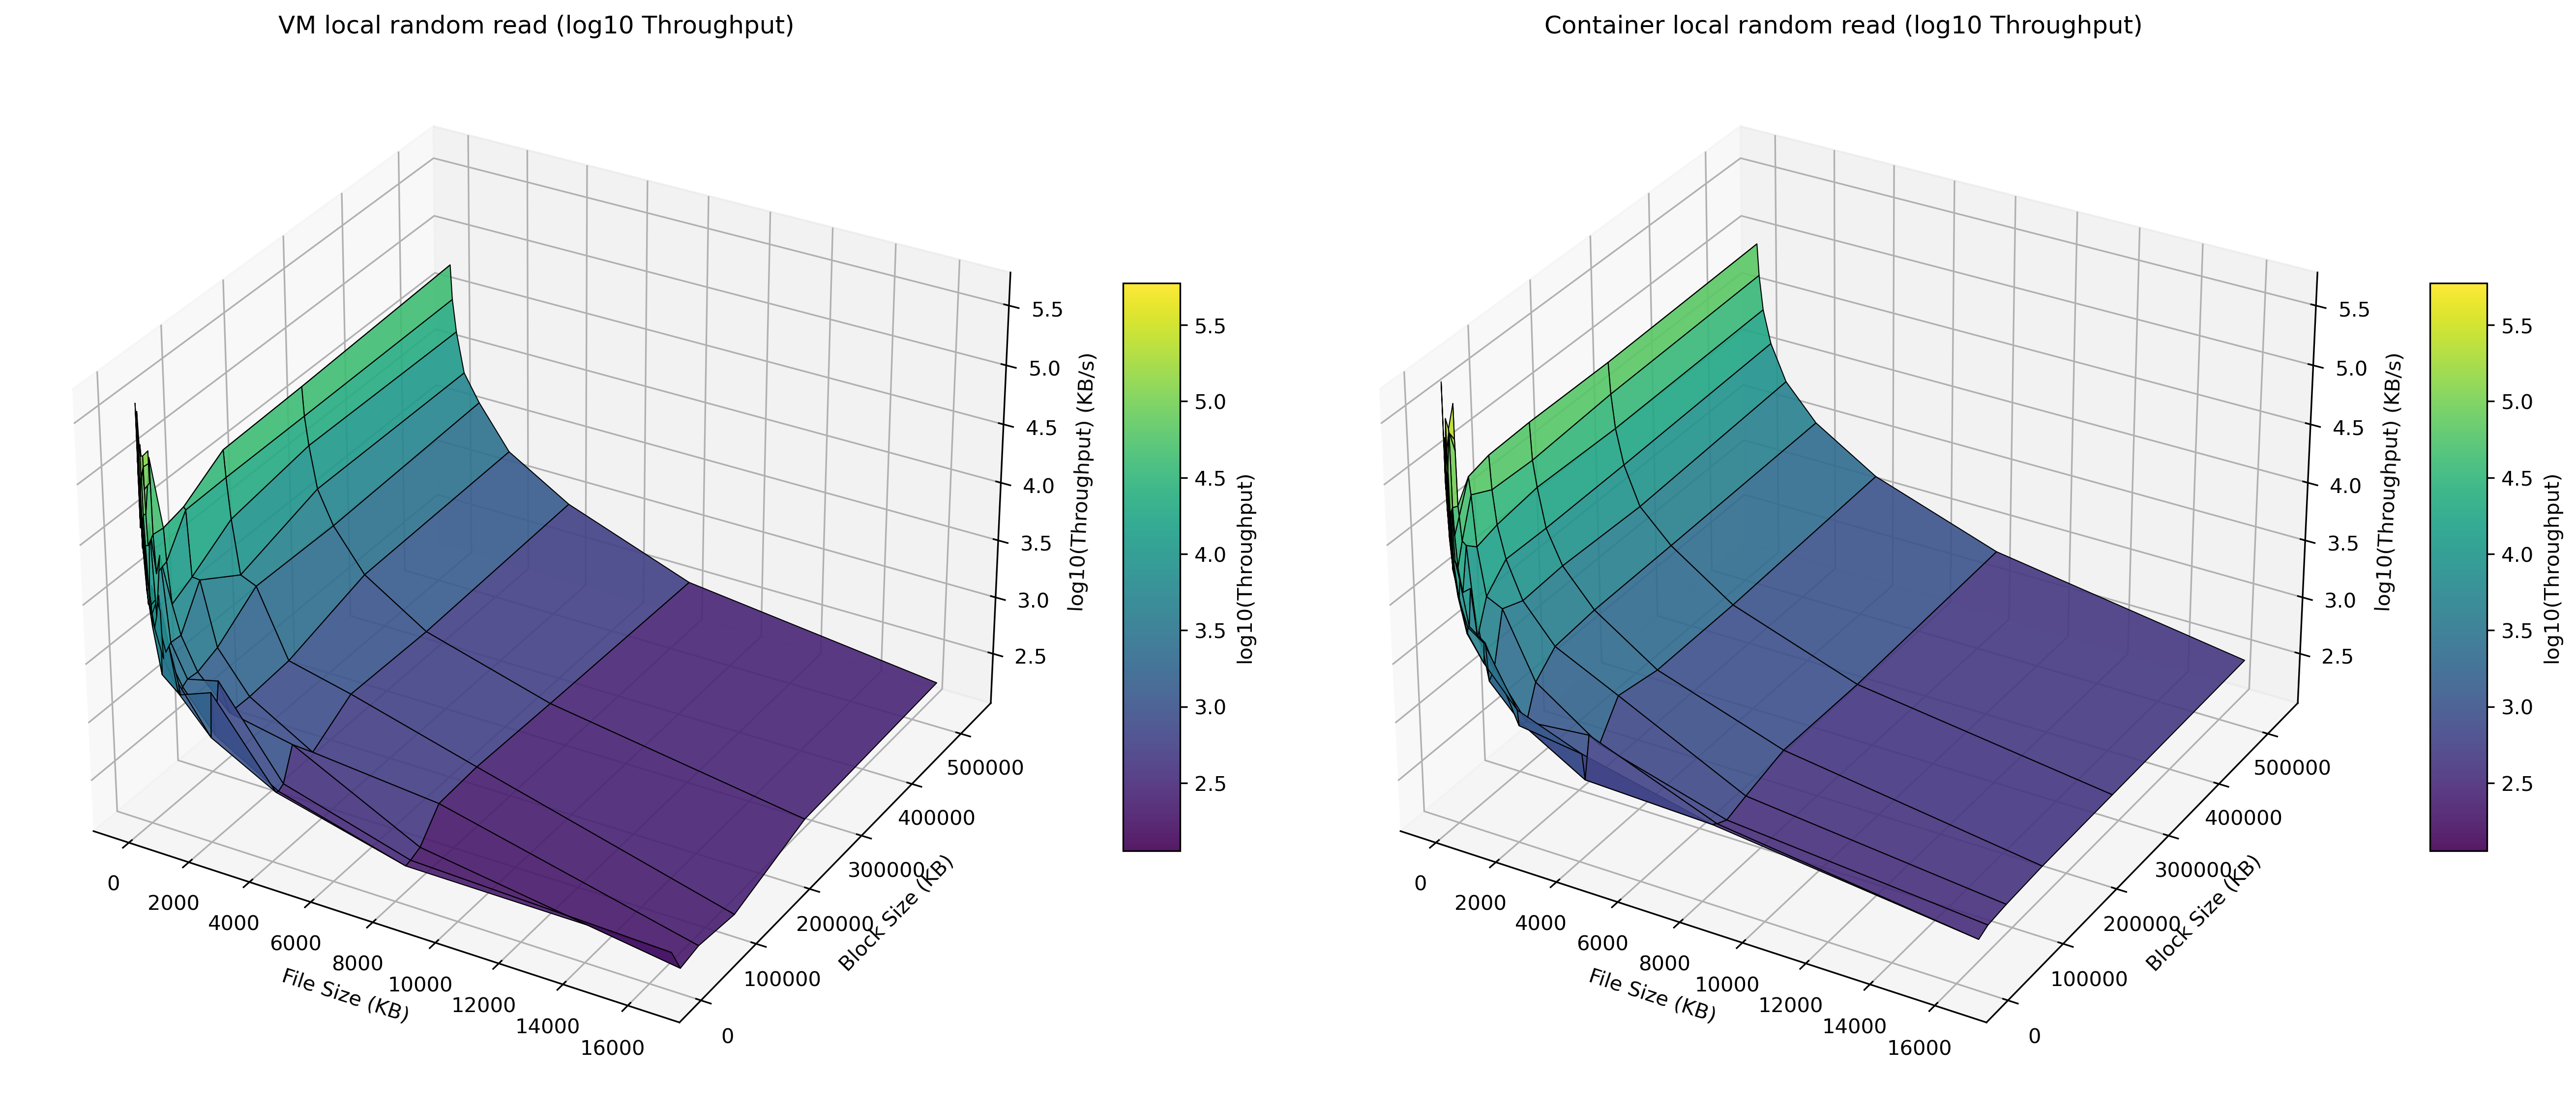
\includegraphics[width=\linewidth]{assets/VM local random read_Container local random read_log_surfaces.png}
        \end{figure}
\begin{figure}[H]
    \centering
    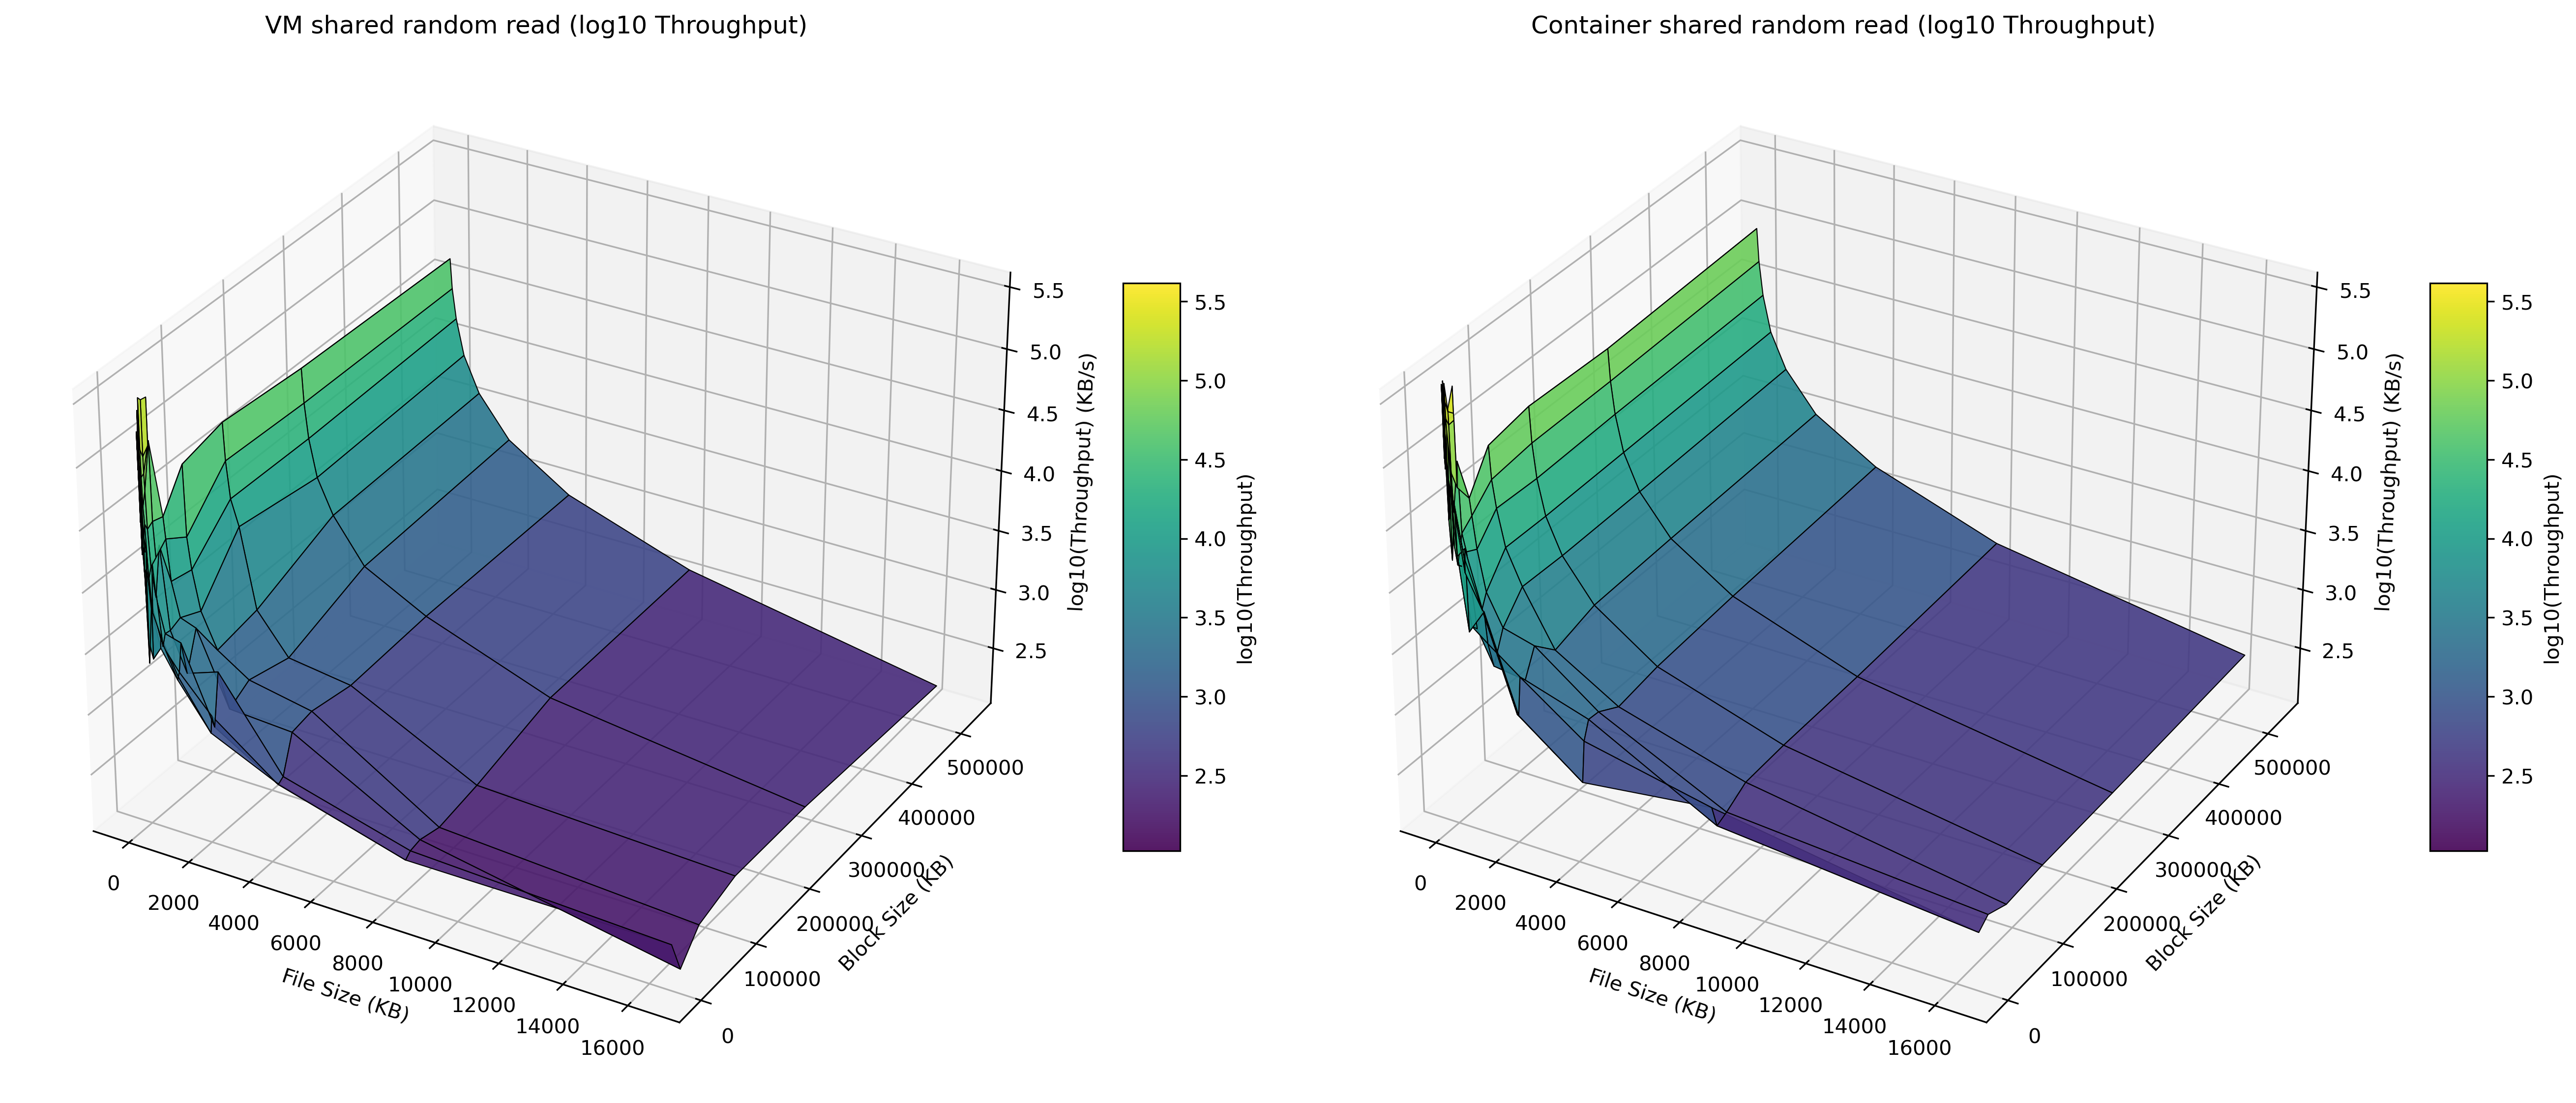
\includegraphics[width=\linewidth]{assets/VM shared random read_Container shared random read_log_surfaces.png}
    \caption{local and shared random read report}
    \label{fig:random read local and shared}
\end{figure}

\begin{figure}[H]
    \centering
    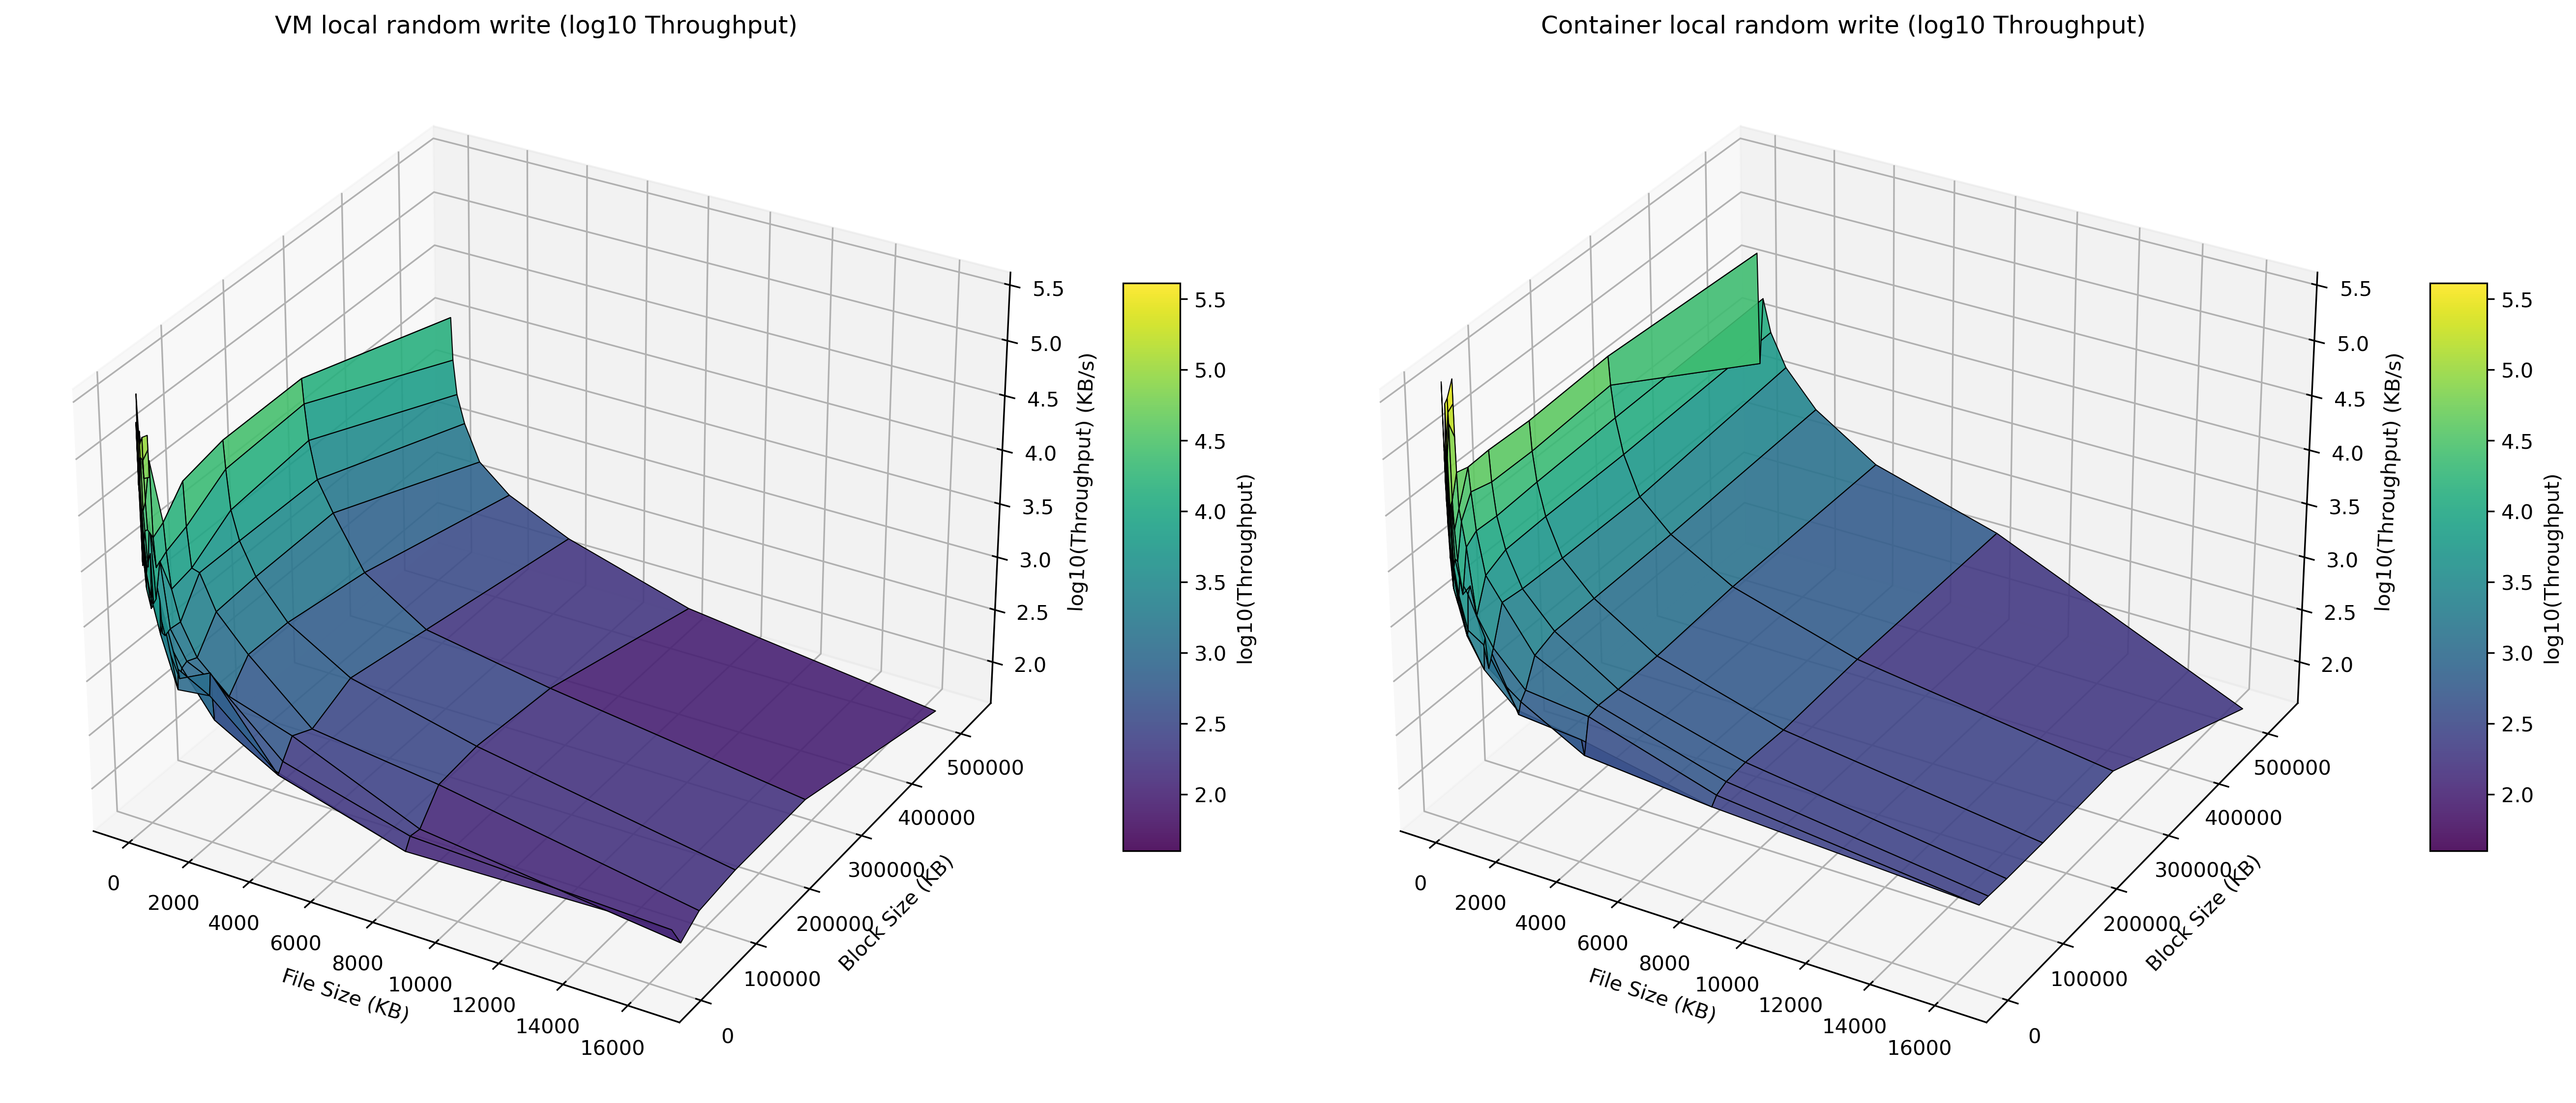
\includegraphics[width=\linewidth]{assets/VM local random write_Container local random write_log_surfaces.png}
        \end{figure}
\begin{figure}[H]
    \centering
    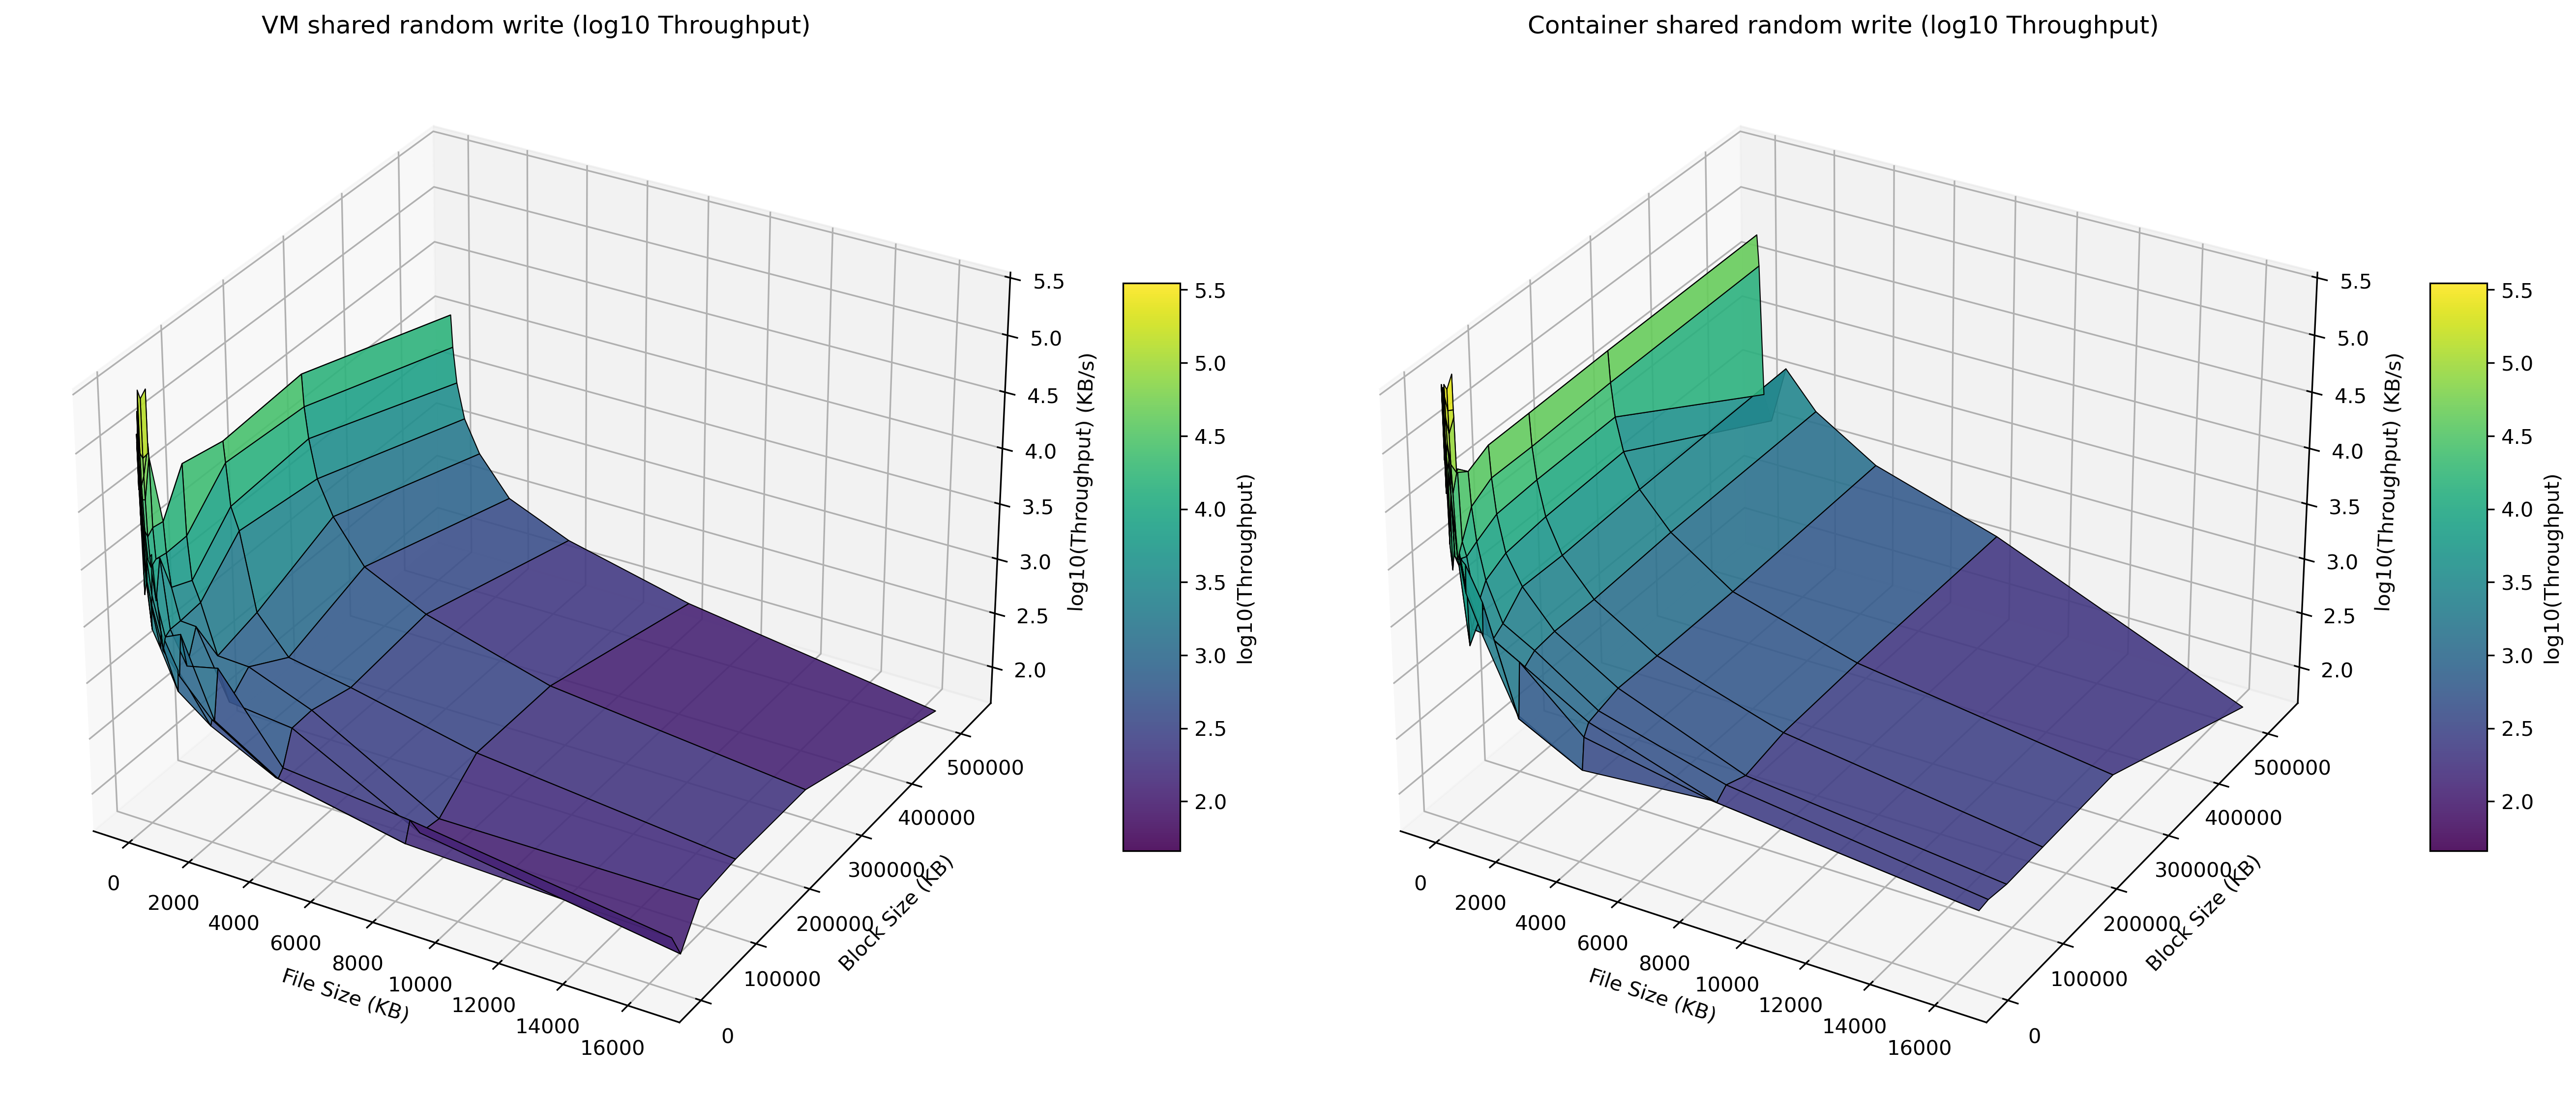
\includegraphics[width=\linewidth]{assets/VM shared random write_Container shared random write_log_surfaces.png}
    \caption{local and shared random write report}
    \label{fig:random write local and shared}
\end{figure}

\subsection{iperf}

iperf is a standard tool used to measure network performance, specifically throughput (bandwidth), latency, and jitter. These results directly assess the quality of the network connection between the nodes in your VM cluster versus the nodes in the Container cluster.

TCP Performance (Upload and Download): 
The bandwidth (Bitrate) is the most striking difference. The Container environment achieves a TCP bitrate of approximately 4.9 Gb/s (both upload and download), while the VM environment is limited to a mere 0.30 Gb/s. This means the network link between the two nodes in the Docker cluster is about 16 to 17 times faster for sustained TCP data transfer than the virtualized network link between the two nodes in the VirtualBox cluster. The Containers are effectively utilizing a much higher bandwidth pipe than the VMs. The relative standard deviations (±) show that the container network performance is not only much higher but also more consistent than the VM network performance.

The iperf results provide the crucial evidence to explain the performance differences observed in benchmarks that rely on inter-node communication. The iperf results definitively confirm the statement that "VMs rely on virtualized NICs with limited performance." The measured TCP bandwidth of 0.30 Gb/s is a severe bottleneck for any distributed application or benchmark (like MPI in HPCC or StarSTREAM) that attempts to send data between the VM nodes. This low network speed directly limits how fast data can be moved between nodes, regardless of how fast the CPUs can process it or how fast local memory is.

The much higher network bandwidth (4.9 Gb/s) and lower jitter in the Container environment explain why the Container cluster would outperform the VM cluster on distributed benchmarks. With a faster and more stable network, the overhead of inter-node communication is significantly reduced, allowing the nodes to exchange data more efficiently and complete the distributed tasks (like those in StarSTREAM or HPCC's MPI components) faster.

\begin{table}[H]
    \centering
    \begin{tabular}{lcc}
    \toprule
    \textbf{Benchmark} & \textbf{VM} & \textbf{Container} \\
    \midrule
    \textbf{TCP upload} & & \\
    Transfer (GB) & $2.66 \pm 0.56$ & $42.48 \pm 6.75$ \\
    Bitrate (Gb/s) & $0.30 \pm 0.10$ & $4.91 \pm 1.11$ \\
    \midrule
    \textbf{TCP download} & & \\
    Transfer (GB) & $2.84 \pm 1.28$ & $43.04 \pm 1.66$ \\
    Bitrate (Gb/s) & $0.30 \pm 0.10$ & $4.97 \pm 0.81$ \\
    \midrule
    \textbf{UDP} & & \\
    Transfer (MB) & $0.12 \pm 0.02$ & $0.13 \pm 0.00$ \\
    Bitrate (Mb/s) & $1.04 \pm 0.08$ & $1.05 \pm 0.00$ \\
    Jitter (ms) & $1.60 \pm 0.74$ & $0.15 \pm 0.08$ \\
    \bottomrule
    \end{tabular}
    \caption{Caption}
    \label{tab:iperf}
\end{table}